%%%%%%%%%%%%%%%%%%%%%%%%%%%%%%%%%%%%%%%%%
% Thesis 
% LaTeX Template
% Version 1.3 (21/12/12)
%
% This template has been downloaded from:
% http://www.latextemplates.com
%
% Original authors:
% Steven Gunn 
% http://users.ecs.soton.ac.uk/srg/softwaretools/document/templates/
% and
% Sunil Patel
% http://www.sunilpatel.co.uk/thesis-template/
%
% License:
% CC BY-NC-SA 3.0 (http://creativecommons.org/licenses/by-nc-sa/3.0/)
%
% Note:
% Make sure to edit document variables in the Thesis.cls file
%
%%%%%%%%%%%%%%%%%%%%%%%%%%%%%%%%%%%%%%%%%

%----------------------------------------------------------------------------------------
%	PACKAGES AND OTHER DOCUMENT CONFIGURATIONS
%----------------------------------------------------------------------------------------

\documentclass[11pt, a4paper, oneside]{Thesis} % Paper size, default font size and one-sided paper

\graphicspath{{./Pictures/}} % Specifies the directory where pictures are stored

\usepackage[square, numbers, comma, sort&compress]{natbib} % Use the natbib reference package - read up on this to edit the reference style; if you want text (e.g. Smith et al., 2012) for the in-text references (instead of numbers), remove 'numbers' 
\hypersetup{urlcolor=blue, colorlinks=true} % Colors hyperlinks in blue - change to black if annoying
\title{\ttitle} % Defines the thesis title - don't touch this

\begin{document}

\frontmatter % Use roman page numbering style (i, ii, iii, iv...) for the pre-content pages

\setstretch{1.3} % Line spacing of 1.3

% Define the page headers using the FancyHdr package and set up for one-sided printing
\fancyhead{} % Clears all page headers and footers
\rhead{\thepage} % Sets the right side header to show the page number
\lhead{} % Clears the left side page header

\pagestyle{fancy} % Finally, use the "fancy" page style to implement the FancyHdr headers

\newcommand{\HRule}{\rule{\linewidth}{0.5mm}} % New command to make the lines in the title page

% PDF meta-data
\hypersetup{pdftitle={\ttitle}}
\hypersetup{pdfsubject=\subjectname}
\hypersetup{pdfauthor=\authornames}
\hypersetup{pdfkeywords=\keywordnames}

%----------------------------------------------------------------------------------------
%	TITLE PAGE
%----------------------------------------------------------------------------------------

\begin{titlepage}
\begin{center}

\textsc{\Large Master Thesis}\\[0.5cm] % Thesis type

\HRule \\[0.4cm] % Horizontal line
{\huge \bfseries Scalable Data Transformation Service for Open Data }\\[0.4cm] % Thesis title
\HRule \\[1.8cm] % Horizontal line


\includegraphics[width=15cm]{Figures/Uni}\\[1.5cm] % University name
 
\begin{minipage}[t]{0.4\textwidth}
\begin{flushleft} \large
\emph{Author:}\\
\href{https://no.linkedin.com/in/nivemaham}{Nivethika Mahasivam} % Author name - remove the \href bracket to remove the link
\end{flushleft}
\end{minipage}
\begin{minipage}[t]{0.4\textwidth}
\begin{flushright} \large
\emph{Supervisors:} \\
\href{http://users.ics.forth.gr/~magoutis/}{Prof. Kostas Magoutis} \\ % Supervisor name - remove the \href bracket to remove the link 
\href{http://www.mn.uio.no/ifi/english/people/aca/dumitrur/}{Dr. Dumitru Roman} 
\end{flushright}
\end{minipage}\\[5cm]
 

\includegraphics[width=9cm]{Figures/Sintef}\\[1cm]
 
{\large \today}\\[4cm] % Date

 
\vfill
\end{center} 

\end{titlepage}


%----------------------------------------------------------------------------------------
%	ABSTRACT PAGE
%----------------------------------------------------------------------------------------

\addtotoc{Abstract} % Add the "Abstract" page entry to the Contents

% \abstract{\addtocontents{toc}{\vspace{1em}} % Add a gap in the Contents, for aesthetics

% }

\clearpage % Start a new page

%----------------------------------------------------------------------------------------
%	ACKNOWLEDGEMENTS
%----------------------------------------------------------------------------------------

\setstretch{1.3} % Reset the line-spacing to 1.3 for body text (if it has changed)

% \acknowledgements{\addtocontents{toc}{\vspace{1em}} % Add a gap in the Contents, for aesthetics

% \noindent The research leading to these results has received funding from the 

% \noindent In addition, I am very grateful to
% }
\clearpage % Start a new page

%----------------------------------------------------------------------------------------
%	LIST OF CONTENTS/FIGURES/TABLES PAGES
%----------------------------------------------------------------------------------------

\pagestyle{fancy} % The page style headers have been "empty" all this time, now use the "fancy" headers as defined before to bring them back

% \lhead{\emph{Contents}} % Set the left side page header to "Contents"
% \tableofcontents % Write out the Table of Contents

% \lhead{\emph{List of Figures}} % Set the left side page header to "List of Figures"
% \listoffigures % Write out the List of Figures

% \lhead{\emph{List of Tables}} % Set the left side page header to "List of Tables"
% \listoftables % Write out the List of Tables


%----------------------------------------------------------------------------------------
%	THESIS CONTENT - CHAPTERS
%----------------------------------------------------------------------------------------

\mainmatter % Begin numeric (1,2,3...) page numbering

\pagestyle{fancy} % Return the page headers back to the "fancy" style

% Include the chapters of the thesis as separate files from the Chapters folder
% Uncomment the lines as you write the chapters

% Chapter 1

\chapter{Introduction} % Main chapter title
\label{Chapter1} % For referencing the chapter elsewhere, use \ref{Chapter1} 

\lhead{Chapter 1. \emph{Introduction}} % This is for the header on each page - perhaps a shortened title

%----------------------------------------------------------------------------------------

\noindent With the bloom of digital data revolution, a plethora of data being collected and shared. Today’s penetrating phenomenon of big data is open data, which is available in liquid format and valued more  than closed data by being shared and accessed\citep{opendataunlockinginnovation}. Making data more liquid essentially means providing open, widely available data in shareable formats \cite{opendataunlockinginnovation}. The openness is ensured by publishing open data in a way that can be understood and used similarly by all users\cite{opendatahandbook}. Main process of open data management includes transforming raw data into a commonly understandable format, sharing or hosting them via a publicly accessible medium, integrating them with other data, visualizing and/or analyzing the data using smarter and simpler queries\cite{howlinkeddataistransforminggovernment}.Despite of the prominent evident in rise of open data era, producing and sharing  open data with required quality remains non-trivial\cite{towardsopendatadevelopmentmodelforlinkeddata} due to lack of fully fledged solutions. 

\noindent Notably, data preparation is a tedious, time consuming step and mostly a compulsory step to receive the optimal value from data in any data processing activity\cite{datapreparationfordatamining}. As the need grows, there are some initiatives who try to provide simpler and easier means for data preparation. However, they address only a subset of open data preparation requirements and/or they are not very simple and cheap solutions\cite{ligthweightopendatatransformation}\cite{cleaningprobsandapproaches}\cite{declarativedatacleaning}\cite{visualizationsandtransformationsinwrangling}. They often require technically skilled resources (to implement domain specific solutions using selected techniques or technologies) and a significant investment of time and money (buying commercial products and maintaining them). Particularly, open data preparation has its unique demand which are not solved to an expected and reachable level yet. In this thesis, we suggest a scalable interactive data transformation as a service based solution especially for open data users. We suggest a solution to do data preparations with interactive user interface that can render data transformation results in near-real-time even for large data-sets. Finally we evaluate it by bench marking it with existing solutions.

%----------------------------------------------------------------------------------------
\section{Background}
Open data and open data management is relatively a new context, the interpretation of few terms are still changing while there is no common agreement of few terms yet.  To avoid ambiguity of the content and to give clear understanding of rest of the content, we discuss few important terms which are often used in this article. 
\subsection{Open Data}
Open data is often derived from the definition of "Open". A material is considered as open \textit{if it is free to access, use, modify, and share - subject, at most, to measures that preserve provenance and openness}. Any open works must satisfy open license or status, access, machine readability and open format\cite{opendefinition}. So do open data. These properties can be reached by introducing  interoperability in data. Interoperability is considered as the ability to be understood and used universally\cite{opendatahandbook}. It is important because it allows different partners to work together on top of agreed commons. In the context of open data interoperability it is vital, as it is the crutch to let different partners to work together. Open data frequently referred as liquid data due to these properties. The liquidity of open data is achieved by publishing in Linked Data format which is mostly called Linked Open Data (LOD). 

\subsection{Open Big Data}
todo

\subsection{Linked Data and RDF Format}
Linked data is the data published on the Web in a way it is machine readable\cite{linkeddatasofar}. The meaning of data is explicitly defined in machine understandable format, then it is linked to the core data. Simply, linked data is data that is connected using typed links from different sources.  Linked data relies on formulating data in Resource Description Framework (RDF) format\cite{rdfdefinition}. 
 
RDF Format : RDF represents a data with a generic graph-based data model\cite{linkeddatasofar} with which to structure data and describe it. RDF model encodes data in the form of subject, predicate, object triples. The subject and object are both URIs or a URI and a string literal to identify respective resources. Predicate mentions the relationship between subject and object, where is also represented by a URI. The resource to describe RDF entities are called vocabularies, which are collections of domain specific classes and properties. RDF Vocabulary Definition Language (RDFS) \cite{rdfsdefinition} and Web Ontology Language (OWL) \cite{owldefinition}  provide the foundation for creating vocabularies. By engaging URIs to identify resources, RDF to represent data resources and HTTP protocol as retrieval mechanism LOD is rendered similar to general architecture of Web which contains a layer of interwoven document data. 

\subsection{Open Data Preparation - Data cleansing and RDF transformation}
Before publishing open data it is important that the data being published is complete, self contained that can be used by anyone. To date, open data are derived from legacy databases, or from static logs, or\cite{collaborativeopendataversioning} in silos of huge Comma Separated Values (CSV) files or Excel spreadsheets\cite{ETL}. These data are typically messy (with errors, missing values, and consistencies) and cannot be immediately transformed into RDF format. Thus data cleansing is important prerequisite for open data preparation before it is mapped to create RDF format. Open data preparation has two main sub-processes such as open data transformation and RDF creation.The usual life-cycle of creation of LOP consists raw data cleaning, transformation (mostly from tabular formats), mapping to ontology and generating semantic RDF graph\cite{datagraftsimplyfyingopendatapublishing}.  This process can be compared to Extract, Transform and Loading (ETL) operations\cite{collaborativeopendataversioning}. The major categories of cleansing and transformation operations are 
\begin{enumerate}
\item Analysis: Data analysis, statistical evaluation and data mining algorithms
\item Profiling: Identify and solve data quality problems (e.g. Misspellings, Cryptic values and abbreviations, Misfiled values and Word transposition) \cite{datacleaningprobsandapproaches}
\item Transformation: Operations to modify the data to fit the target schema (e.g. Embedded value,  Duplicate records, Pivoting and Un-pivoting, Slowly Changing Dimensions (SCD), Surrogate keys)\cite{datacleaningprobsandapproaches}\cite{ETL}
\item Cleaning: Detecting, removing and correcting dirty data together with schema-related transformation based on comprehensive meta-data (e.g. String problems). \cite{datacleaningprobsandapproaches}
\item Duplicate elimination: Identifying and merging duplicate records (e.g. Full duplicates and grouped duplicates)
\item Enrichment: Using additional information to improve data quality (e.g. Surrogate keys, SCD)\cite{ETL}
\end{enumerate}
These are typically needed in most of the transformation tools. However, for our case we consider analysis as rather a post step where a fully fledged analysis can be performed on top of integrated RDF data. The rest of the five categories are mostly used to help user to create a perfect 'fit for purpose' data from messy data. 

\section{Research Motivation}
The hype of "open data movement" made many governments and non-profit organizations(NGO) to publish their data. Nevertheless, the published data remains ineffective since it is nonfunctional without prescribed interoperability. Statistics says that 80\% of data in publicdata.eu which aggregates data from 30 European data portals are in tabular formats (Excel sheets or CSV files)\cite{nemreport}. In addition only 1\% of published data are presented with vocabularies and presented in RDF format\cite{nemreport}. Next generation research questions can be answered only by integrating data from different sources\cite{nemreport}. This brings the ultimate goal of open data movement unsettled. Especially, how large open data can be processed to provide liquid data is unresolved. Data preparation of big-open data becomes the "\textit{enabler}" of active open data analysis. The way out from this is to enable easy data transformation from legacy data to liquid format. 

\noindent  Open data workers are not essentially technically oriented. Data workers reported spending more than 80\% of their development time in data cleaning\cite{visualizationsandtransformationsinwrangling}\cite{Wisteria}\cite{journals/corr/KrishnanW0FG16}. Often data preparation requires writing idiosyncratic scripts like Python, Scala, Perl and R or engages tiresome manual editing. Survey says this discourages a large number of workers from working with data, as well as they spend most of their time dealing with data rather than excelling in their desired sector\cite{visualizationsandtransformationsinwrangling}. This highlights on a crucial user friendly solution.

\subsection{Escalated Challenges}
\textbf{Repeatable and Reusable cleaning}: The cleanness or quality of data data can't be decided upfront. The correctness and effectiveness of a transformation work-flow should be verified(execute on a sample of data and improve the workflow definition if necessary). Data cleaning can bring new quality issues iteratively while being cleaned. Thus, data cleaning is an inherently iterative procedure\cite{Wisteria}. A data cleaning process should be repeatedly applicable on data and provide incremental output. Data cleaning may involve trail and error instances\cite{visualizationsandtransformationsinwrangling}. A data worker should be able to roll-back to desired stage whenever required. Furthermore, same transformation process can be performed on multiple data-sets. Importantly, when a data cleaning is crowd-sourced important of capturing data alterations is heighten\cite{2011-wrangler}.  Hence, it is must to keep record of how a data had been processed during cleaning process in share-able format. 

\textbf{Interactive cleaning}: A data worker must be able to review and refine the cleaning process seamlessly. Visual analytic research\cite{Keim08visualanalytics:} proves that tight visual interaction with user helps to unseat errors easily and quickly. Especially visualization of data helps to immediately eliminate missing values, inconsistencies and wipe out outliers\cite{visualizationsandtransformationsinwrangling}.  In open data analysis a spreadsheet-like interface suits well representing a relational table structure. This enable self-serviced data transformation process. Visualization of data cleaning process is also equally important and should be performed by general audience. It is vital that transformations can be performed just by using a self-contained user interface components than manually writing scripts. 

\textbf{Responsive in near-real-time  and Sampling}: Interactive data transformation directly derives the need for real-time responsive user interfaces. This is possible for small data. However, processing a large data takes significant time that may be accumulated to a noticeable duration for the whole process. This will make the interaction harder and inefficient. For example, considering a scenario when a cleaning operation was performed wrongly and rolled-back, this leads to a significant waste of resources if executed on big data. Big data requires rethinking of current processes\cite{nemreport}. Correctness and Efficiency are important facets of data cleaning\cite{journals/corr/KrishnanW0FG16}. Sampling data-sets is a well-known technique of data cleaning and analysis\cite{Hellerstein08quantitativedata} for various purpose. This can be exploited in iterative data cleaning. Processing streams of small data groups can help when the data is not considered as a single batch input\cite{nemreport}. Sequential sampling (fetching an ordered subset) and random sampling (fetch subset from randomized data) can help for batch inputs. However, improper sampling can lead to wrong decisions\cite{journals/corr/KrishnanW0FG16}. For example a quantitative data may not able to spot outliers correctly if it is sampled sequentially. It will produce more accurate data if it is sampled randomly\cite{Hellerstein08quantitativedata}. Thus, a feasible mechanism to decide on sampling should be available. There is a gap in the literature to pinpoint a proper mechanism to sample data for iterative data cleansing. Few platforms\cite{2011-wrangler} \cite{Wisteria} uses sampling for interactive data cleaning. But the sampling method is unknown to the user and user is not given a choice to choose sampling mechanism.

\textbf{Availability}: Even though data cleaning is just one big step in data analysis process, it is not an instant process. A user should be able to perform consecutive transformation on system for longer duration. The system should not have a single point of failure\cite{mesa}. Cloud computing and distributed computing paradigm has proven solutions for availability issues. Providing solutions as a service enables more availability and waives complex installation and maintenance costs.

\textbf{Scalability}: As we mentioned earlier open data can be small or big. The system must be able to scale according to the size of data. Currently available data cleaning solutions such as OpenRefine\cite{openrefine} and Wrangler \cite{2011-wrangler} are desktop applications, which cannot process bigger data. Further, they allocate large amount of local computing resources which doesn't allow any other operations to be performed on hosted system. This augments the need for a distributed solution of open data preparation. 

\textbf{Separation between logical and physical implementations of data cleaning work-flow}: Most of the interactive data cleaning tools don't have clear separation of their logical and physical implementation of data transformation activities\cite{declarativedatacleaning}\cite{Wisteria}. In many case ETL work-flows are defined in high-level languages\cite{ETL}. This ceases from exploiting the logical query optimization. This is substantially results in inefficient and high-cost transformation work-flow for bigger data.  Logical query optimization is not possible unless otherwise the data worker consciously designs the cleaning work-flow accordingly\cite{ETL}. A automated mechanism to optimize cleaning work-flow can improve performance. 

\textbf{Single ended solution}: The main problem that hasn't been solved is a single endpoint for open data preparations. The system should be able to support data cleaning and transformation to RDF format seamlessly. The existing solutions focuses only on a subset on problem. KARMA \cite{karma}, LinDa project tools\footnote{http://linda-project.eu/} focuses only on formulating linked data from tabular formats whereas many other leading commercial tools such as IBM DataWorks\footnote{http://www.ibm.com/analytics/us/en/technology/cloud-data-services/dataworks/} , Talend Open Studio\footnote{https://www.talend.com/products/talend-open-studio} and Pentaho Kettel \footnote{http://wiki.pentaho.com/} are focusing only on data cleaning processes. They also lack few of the open data cleaning techniques discussed above. Open data workers need an integrated and simplified solution that can help them produce quality liquid data which is in high demand nowadays. 

\section{Motivating Scenario(DataGraft)}

\section{Research Problem}

\section{Research Questions}

\section{Research Method}

Other requirement.
Transformation Mapping functions should be declarative and should be reusable for other data.especially a workflow transformation structure  should be supported execute all data transformation steps for multiple sources. Schema level transformation and cleaning should be specified by declarative query and mapping language as far as possible, to enable automatic generation of the transformation code. It should be possible to invoke user-written cleaning code and special purpose tools during a data transformation workflow.  transformation steps may request user feedback . auto duplicate elimination and schema matching.
Verification: The correctness and effectiveness of a transformation workflow and the transformation definitions should be tested and evaluated, e.g., on a sample or copy of the source data, to improve the definitions if necessary
more work is needed on the design and implementation of the best language approach for supporting both schema and data transformations.operators such as Match, Merge or Mapping Composition have either been studied at the instance (data) or schema (metadata) level 

Most of the data transformation tools don't have clear separation of logical specification of data transformation and physical implementation. \cite{declarativedatacleaning}
todo: current systems support limited data cleaning support focusing on transformation and schema translation. should provide more support to data cleaning. data must be extracted from multiple sources and transformed n combined  during query time.  

Why better than existing ETL tools? in usual ETL workflows transformations are mentioned in high-level-language. Logical query optimization is not possible unless the user designs it with consideration upfront\cite{ETL}. Lot of work for designer. Now spark catalyse code generator transforms pipe into optimized logical queries. 

Questions: Can we use espemino as sample and ask them to give bigger data? 
The dataset used to show in uio seminar by titi
% As the need for open data sharing is increasing, there are some  initiatives that try  solve these needs. However, such initiatives only address a subset of needs such as either data cleaning or transformation (or any other combinations of the activities in the data sharing process\textbf{ confusing??/)}.  In this thesis, we explore how can we provide a scalable open data sharing needs as a service by eliminating current limitations. 


% \section{Research Motivation}

a comparative study on leading solution providers

% Definitions  
% Open data 

% Linked data 

% Data tranformation in open data : combination of data cleanging and transformation it to RDF

% Data cleaning 
% Scalable

% Near real time 
% Interactive transformation 

% Linked Data
% Open data is commonly shared in Linked Data format, which is defined as a set of best practices for publishing and connecting structured data on the web\cite{linkeddatasofar}.  Open governments, public administrations and other commercial organizations have recently started publishing large amount of structured data. There 

% Open data is the data that can be used, re-used and redistributed by anyone without any limitations or at minimal limitations\cite{opendatahandbook}. 


% %----------------------------------------------------------------------------------------

% \section{Research Motivation}

% In this section we outline several reasons how the research presented in this paper  addresses important concerns of 
% related work 
% explain the archi
% open refine
% karma
% trifacta
% ibm dataworks
% talent 
% lightweight transformation of tabular open data to rdf
% similar solutions address the domain and what they lack and how they are related to our work


% \subsection{Background}

% \noindent As we mentioned earlier, important challenges during 

% %----------------------------------------------------------------------------------------

% \subsection{Motivating Scenario}
% DataGraft.net, a cloud based open data sharing platform tries to address all these needs together as a service. However, it has limitations of transforming large data.
% \noindent To have a better understanding of the previously discussed challenges and approaches, the following motivating scenario has been developed: 
% introduce datagraft in detail, how it address the common needs in big picture. 
% architecture
% todays limitations in data transformation.


% %----------------------------------------------------------------------------------------

% \subsection{Discussion}
% \label{sec:Discussion}
% why this limitation
% who eliminating this can help 
% what is expected from this?

% %----------------------------------------------------------------------------------------

% \section{Research Problem}

% \noindent In this work we focus on two challenges: (i) combination of the declarative and imperative approaches to the application provisioning and deployment, and (ii) continuous deployment of cloud applications. Based on this, the research problem may be formulated as follows: 

% How to transform larger data without technical knowledge
% how interactive transformation of large files can be done in near-real-time?

% \begin{center}
% "How can we enable both, flexibility and fine-grained control, in the deployment and provisioning of multi-cloud applications, and allow efficient run-time management of such applications?"
% \end{center}

% \section{Research Questions} 

% \noindent The problem addressed by this thesis rises the following questions:

% \begin{enumerate}
% \item  How imperative and declarative approaches can be combined? Does a combined approach furnish a more efficient and flexible solution?

% \item  How to create a DSL for the specification of deployment plans that can be used in combination with declarative deployment topology models, and programmatically by a third party?

% \item  How such DSL could be used to support efficient continuous deployment of multi-cloud applications?

% \end{enumerate}

% %----------------------------------------------------------------------------------------

% \section{Research Methodology}
% In this section we explain our research methodology and develop a research work plan.

% %----------------------------------------------------------------------------------------
% \subsection{Methodology}

% \noindent The adopted methodology of this thesis relies on a literature survey and design science \cite{von2004design}. Literature survey covers not only publications in scientific journals but also analysis of widely used tools because provisioning and deployment processes relate more to the practical side of computer science than its theoretical underpinnings. Design science guidelines help us in the development of our solution and ensuring that our results are relevant, verifiable and appropriately evaluated.

% %----------------------------------------------------------------------------------------
% \subsection{Work Plan}
% Following the discussion from the Section \ref{sec:Discussion} and, according to the research problem, we can define the initial set up for the research: the approach that we will work on must be declarative, open source and provide support for the continuous deployment. Then, the work plan to answer research questions includes the following steps:

% \begin{enumerate}
% \item  Analyze state of the art tools and approaches for 

% \item  Choose a declarative approach for the improvement.

% \item  Analyze how deployments plans are defined in imperative approaches. Extract common characteristics and limitations of languages used to define deployment plans, and create a domain-specific workflow definition language to specify such plans.

% \item  Integrate a chosen approach, including the continuous deployment functionality, with created DSL.

% \end{enumerate}

% \noindent The rest of the thesis is organized as follows. In Chapter 

% solution analysis - state of the art spark
% Dataframe 
% feasibility test
% dataframe performace tests
% https://databricks.com/blog/2015/02/17/introducing-dataframes-in-spark-for-large-scale-data-science.html

% https://0x0fff.com/spark-dataframes-are-faster-arent-they/

% implementation - Scalable transformation of open data

% problem
% archi- should explain clearly for backend n front-end 
% solution components
% sparker
% scalable-graftwerk
% grafterizer
% deployment - possible on local and cluster 

% evaluation

% Integration n usability

% functional coverage- how much persisted from earlier, how much can be added newly
% consistency-
% reliability - no sandbox
% scalability
% availability

% Performance evaluation

% experiment setup

% of single machine - oldgraftwerk , sparker on local, open refine

% for different file size, same pipeline

% trifacta, open refine, setup on cluster

% conclusions
% posible transformation for big data. without limitation. can be hosted in local cluster is provided service is not enough. the limitation is eliminated. 
% technical contributions
% scientific contributions

% appendix


%----------------------------------------------------------------------------------------
% % Chapter 2

\chapter{Literature Review} % Main chapter title
\label{Chapter2} % For referencing the chapter elsewhere, use \ref{Chapter2} 

\lhead{Chapter 2. \emph{Related work}} % This is for the header on each page - perhaps a shortened title

%----------------------------------------------------------------------------------------
\section{Escalated Requirements in Domain}
\label{sec:requirements}
In this section, the important requirements identified which should be solved by an integrated open data preparation solution are discussed. 
\textbf{Reusable and Repeatable cleaning }
The same transformation process can be performed on multiple data-sets. Importantly, when a data cleaning is crowd-sourced, the need for capturing data alterations is increased\cite{2011-wrangler}.  Hence, the solution must keep track of how a data had been processed during the data cleaning process and should be share-able. 

\subsection{Real-time responsive architecture}
\noindent Interactive data transformation directly derives the need for responsive user interfaces. This is possible when data being processed is small. For example, OpenRefine \cite{openrefine}  is an interactive featured open data cleanser can process only small volumes of data, whereas the size of the data that need to be processed growing exponentially. The root cause for this issue is these systems are not considered to be effective on large volume of data during design and implementation state. It is of utmost important that the next generation solutions should be considered to process large volumes of data from designing stage itself. There is no disclosed architecture or an efficient and effective work-flow which can work with real-time interactive cleaning on large data.  An optimized process that should work for big data cleaning in real-time should be considered and implemented by proposed solution. 
\subsection{Sampling}
\noindent Processing a large data takes significant amount of time that may be accumulated to longer duration for the whole multi-step process. This will make the interaction harder and expensive. For example, considering a scenario when a cleaning operation was performed wrong and rolled-back, this leads to a significant waste of resources if it was executed on large data. Big data processing requires rethinking of traditional processes \cite{nemreport}. Correctness and efficiency are important attributes of data cleaning \cite{journals/corr/KrishnanW0FG16}. Sampling data-sets is a well-known technique of data cleaning and analysis \cite{Hellerstein08quantitativedata} for various purpose. This can be exploited in interactive and iterative data cleaning. Sequential sampling (fetching an ordered subset) and random sampling (fetch subset from randomized data) can help for large inputs. However, improper sampling can lead to wrong decisions \cite{journals/corr/KrishnanW0FG16}. For example a quantitative data may not able to spot outliers correctly if it is sampled sequentially (e.g. subset of first-N rows and calculate the average of sample). It will produce more accurate data if it is sampled randomly \cite{Hellerstein08quantitativedata}. There is a gap in the literature to pinpoint a proper mechanism to sample data for iterative data cleansing. A data cleaning platform Wisteria \cite{Wisteria} and data integration tool KARMA  \cite{knoblock15:aimag} use sampling for interactive data cleaning. But the sampling method is unknown to the user and user is not given a choice to choose sampling mechanism.  Thus, a feasible mechanism to decide on sampling should be available to the user.
\subsection{Availability and Accessibility}
\noindent Data preparation is not an instant process. A user should be able to perform consecutive transformations on a system for long duration. The system should not have a single point of failure \cite{mesa}.  In addition, in open data field, crowd-sourced data cleaning and transformation is getting popular which are called \textit{Multi-sector planning and analysis} \cite{multisectoranalysis}. It requires collaborative transformations, i.e. a data cleaning and transformation done by multiple partners. Pure offline applications hinders collaborative transformations. Cloud computing and distributed computing paradigm has proven solutions for availability issues. Providing solutions as a service enables more availability and waives complex environment installations and maintenance costs. This emphasis the need of an online data preparation application that can be shared-accessed and available between group of people.
\subsection{Separation between logical and physical implementations of data cleaning work-flow}
\noindent Most of the data cleaning tools don't have clear separation of their logical and physical implementation of data transformation activities \cite{declarativedatacleaning}\cite{Wisteria}. Typically ETL work-flows are defined in high-level languages \cite{ETL}. This ceases from exploiting the logical query optimization which substantially results in inefficient and high-cost transformation work-flow for bigger data.  Logical query optimization is not possible unless otherwise the data worker consciously designs the cleaning work-flow accordingly \cite{ETL}. An automated mechanism to optimize cleaning work-flow can improve performance of data cleaning. 
\subsection{Flexibility}
\noindent Interactive data cleaning and transformations are often supported by underlying Domain Specific Languages (DSL) \cite{Wisteria}. They are typically less exposed and strongly typed. Although, the proposed system should support non-technical workers to do data cleaning, the optimal value can be achieved if the flexibility is given for customized transformation for technical users. 
\section{Related Works}
\label{sec:relatedwork}
Related works which fall under the categories of linked data and open data preparation and ETL tools are discussed in following section. The most relevant systems are discussed with distinctive features highlighted.
\subsection{OpenRefine}
OpenRefine is the most relevant tool regarding the functional requirements of this work, allows to load, understand, clean, reconcile and augment data\footnote{https://github.com/OpenRefine/OpenRefine/blob/master/README.md}. OpenRefine, which was originally GoogleRefine, provides support for both data cleaning and RDF mapping and transformation using RDF Refine plugin, with an interactive user interface. OpenRefine is developed in Java and Jetty that runs locally on host machine as a desktop application. It is inefficient with large data volumes since it implements multi-pass approach \cite{onestopshotforopendata} which consumes large amount of computing resources while executing. It doesn't scale with the size of data. In addition, being an offline desktop application it cannot support collaborative cleaning and transformation.  BatchRefine\footnote{https://github.com/fusepoolP3/p3-batchrefine} is a collection of wrappers that provides support to run OpenRefine in batch mode. However, it has some limitations such as should be executed from command-line, lack of features implemented to support distributed processing, complex installation. This introduces complexity of execution via scripts which required technical knowledge. Further, neither OpenRefine nor BatchRefine were developed with component based architecture, results in tight coupling of core components. This prevents users from reusing this implementation for newer requirements. The proposed system aim to overcome these problems by providing a single ended, large scale open data preparation tool as a service.  
\subsection{Trifacta's Wrangler}
Wrangler is a data cleaning software, provided as a limited desktop application that provides interactive user interfaces to preview data cleaning results in real time \cite{2011-wrangler} \cite{visualizationsandtransformationsinwrangling} \cite{Keim08visualanalytics:}, currently process up to maximum 100 MB data, provided by Trifacta. Wrangler Enterprise\footnote{https://www.trifacta.com/products/wrangler-enterprise/} is an expensive, commercialized application that can support data cleaning in large scale using pipelines supported by Spark or MapReduce. However, main impediment seen in Wranger is, it purely concentrates on data cleaning without any support for linked-data preparation. In addition, Wrangler focuses only on single data cleaning and requires user to manually write domain specific scripting to perform data cleaning which requires learning of related scripts. Further, Wrangler is a desktop application, doesn't support collaborative transformation, reusing or sharing of transformation. By providing a service based solution that can process data cleaning, transformation and integration on large data with interactive user interfaces, the proposed solution is expected to be more useful for open data workers. 
\subsection{KARMA}
KARMA\footnote{http://usc-isi-i2.github.io/karma/} is a data integration tool, built by University of Southern California, that helps mapping structured data into semantic web data, also called as linked data \cite{karma}. KARMA supports integration of data from various sources. It allows users to 1) import data from wide variety of data sources, 2) clean and normalize data, 3) quickly build a semantic description of data  4) integrate data using those semantic models \cite{knoblock15:aimag}. KARMA is one of the main inspiration of this work. However, KARMA focuses on schema level integration, but not record level integration. Specially, KARMA is not a cloud based application, which hinders execution on very large volume \cite{knoblock15:aimag} as well as KARMA focuses on volume by executing transformation on sampling, but doesn't concentrate on data velocity. The proposed system is a cloud based solution and aimed to model the high level cleaning and transformation engine independent from data velocity such that can easily support data streaming and micro batching if necessary. 
\section{Discussion}
A simple comparative analysis was done on aforementioned relevant systems to distinguish the importance of proposed system. Table \ref{tab:2} shows the comparison between those systems and proposed solution. This proves that proposed solution has significant relevance and resolves important issues in the domain. 
\begin{center}
	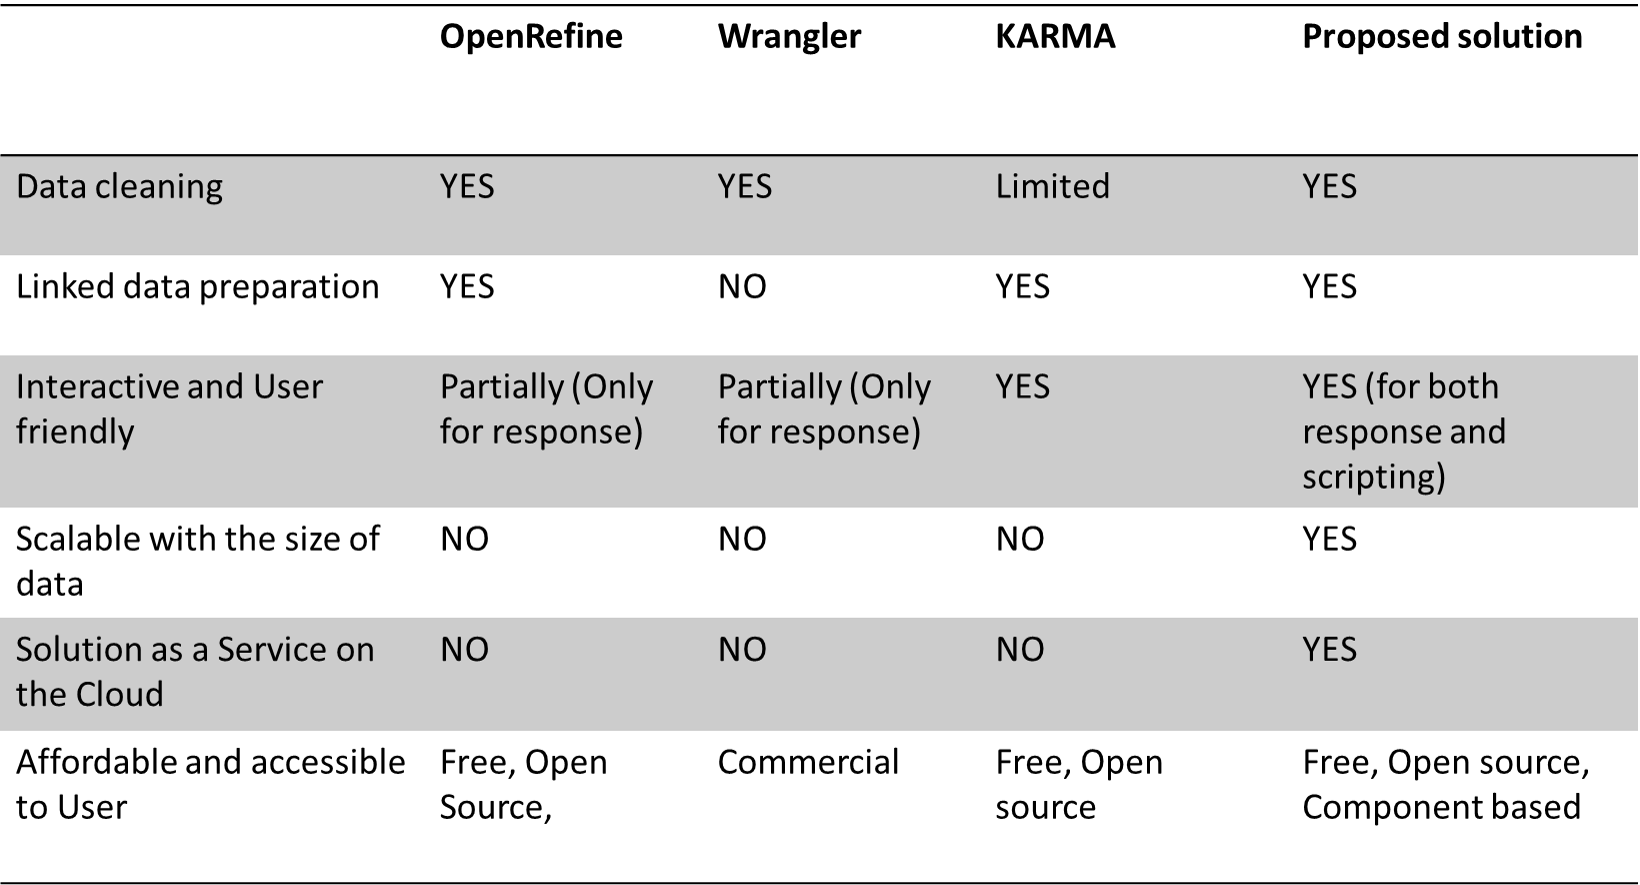
\includegraphics[width=38em]{./Figures/comparative_analysis}
	\begin{table}[htbp]
    \caption{Comparative analysis on relevant systems}
    \label{tab:2}
	\end{table}
\end{center}
 
% % Chapter 3

\chapter{State-of-the-art Analysis} % Main chapter title
\label{Chapter3} % For referencing the chapter elsewhere, use \ref{Chapter3} 

\lhead{Chapter 3. \emph{State-of-the-art Analysis}} % This is for the header on each page - perhaps a shortened title

%----------------------------------------------------------------------------------------
In this section, we discuss the core requirements and other factors that are required to be solved to provide a viable solution. There are plenty of alternatives available under each topic. Thus, we consider solutions that are mostly relevant, widely available and used in the related domain, industry as well as findings from latest related research works. This analysis enables us to choose the best data treatment technique and programming model that are well suited and to select the core design aspects that need to be considered. To make selections with adequate foundation, we first discuss the requirements and then compare each alternatives with respect to the requirements. 
\section{Fundamentals }
\label{sec:fundamentals}
Essential requirements that need to be met by the system are defined in Section \ref{sec:motivation} and additional aspects that needs to be solved by new scalable ETL tools are mentioned in Section \ref{sec:requirements}. To summarize, the system should be execute data preparation on large data (R1), scalable i.e. able to distribute the work according to the load  (R2), real-time responsive in interactive context (R3), efficient on iterative execution (R4). Further, Separation between logical and physical implementation of data cleaning operations becomes an optimization requirement (R5), providing flexibility (R6) behaves as a functional improvement requirement and solution as a service (R7) to provide a general integral solution.  The following important topics need to be carefully analyzed with respect to problem space to create a fit-for-purpose solution. 

\subsection{Data ingestion technique}
Data ingestion technique is a data processing model or the routine how the input data is initially received and represented to be processed. The most frequently used data ingestion or treatment techniques in big data paradigm are batch processing, stream processing and micro-batch processing \cite{dataflow}. Batch processing is a technique of treating the input data as a collection of data where the input data is assumed as fully available to be processed \cite{Sims-387}. Batch processing is generally used as store-first, process-second model of large and of identical types. In contrast, stream processing is a data processing model where data is treated as streams of data \cite{beyondbatchprocessing}. For example, a data stream can be generated based on event-by-event or complex-event-streams. They are not considered to be pre-available before it is processed and they can be out-of-order, out-of-streams \cite{beyondbatchprocessing} \cite{Sims-387}. Stream processing is mainly aimed to do continuous processing on similar data streams in real-time \cite{8reqofrealtime}. Micro-batching is a combined version of batch processing and stream processing, which is to treat data as sequence of small batches of streams. Streams can be delayed to collect small batches or batch inputs can be split into small set of streams to become micro-batches. 
\begin{center}
	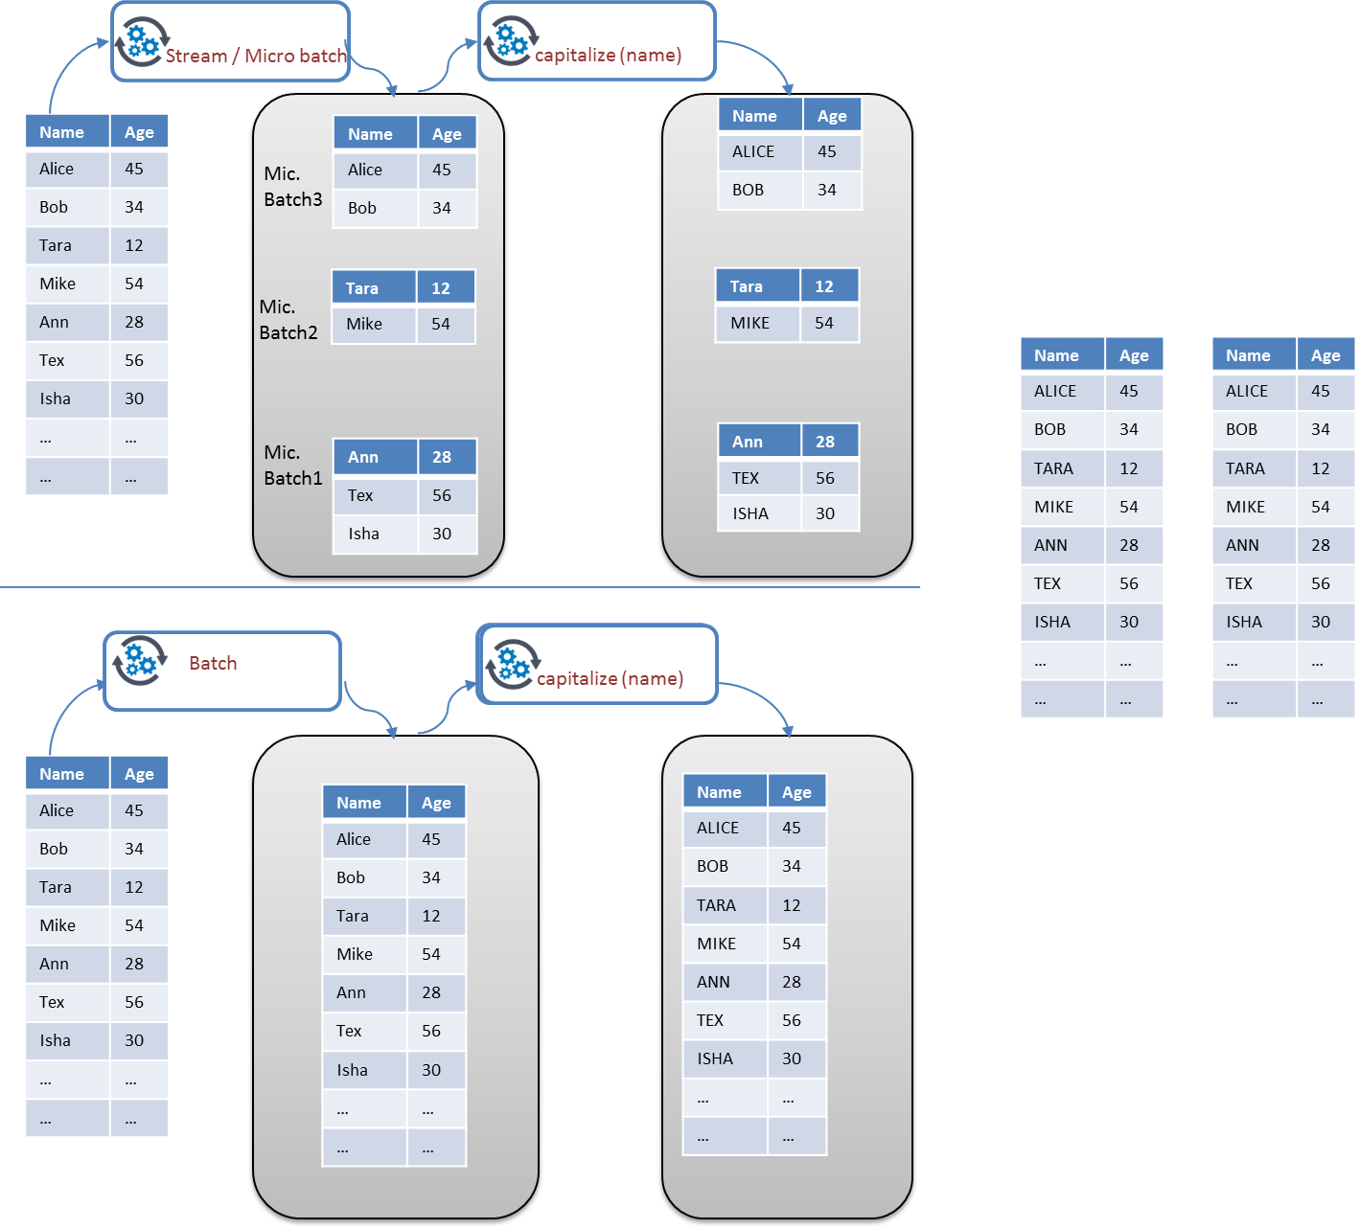
\includegraphics[width=38em]{./Figures/batch-cleaning-right}
	\begin{figure}[htbp]
    \caption{Data cleaning in different data treatment techniques performed as expected}
    \label{fig:streamcorrect}
	\end{figure}
\end{center}
 On small intervals, the incoming stream is collected to a chunk of data and delivered to be processed as a small batch of input \cite{beyondbatchprocessing}. 
 
 Choice of appropriate data ingestion technique is essential to receive precise output. Given that, on today's date, the messy data we target to process in open data context are usually text-files or spreadsheets. These data are already available and need to be processed to create RDF data. 
 Since we need to process large files, the right choice of data ingestion is important. Streaming or Micro batching data can be a solution to overcome the problem of processing large files. However, since we need to perform ETL operations on table like data, it will not result in expected output in all instances. Figure \ref{fig:streamcorrect} shows that streaming or micro batching can provide expected solution when simple data cleaning operations performed independent from other row values such as capitalize, lower case and upper case etc. 
 \begin{center}
	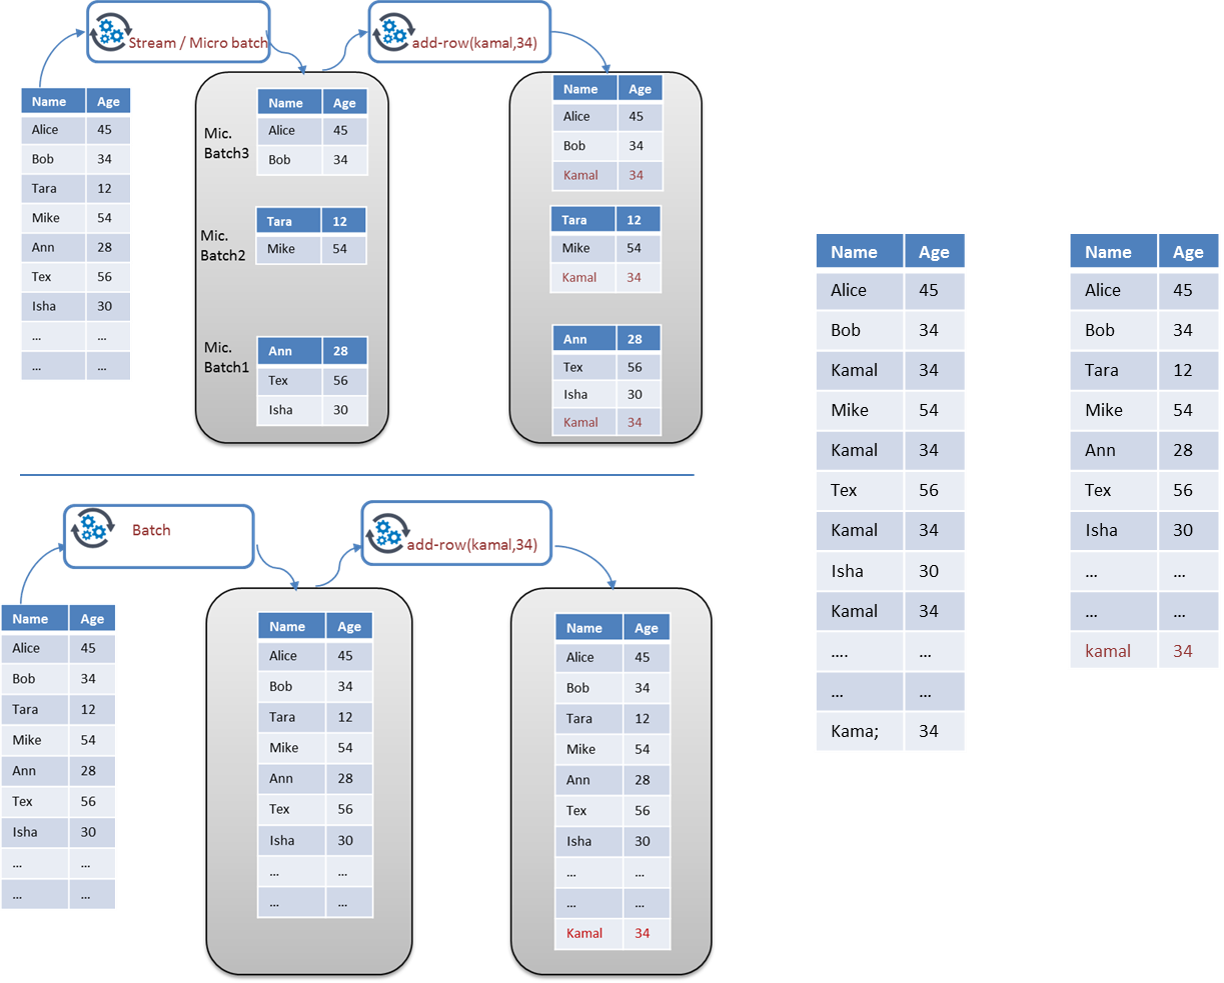
\includegraphics[width=38em]{./Figures/batch-cleaning-wrong}
	\begin{figure}[htbp]
    \caption{Data cleaning on a faulty data treatment results in unexpected result}
    \label{fig:stream-wrong}
	\end{figure}
\end{center}
 However, it will result in wrong output when collective operations or row dependent operations like add-row is performed on data as shown in Figure \ref{fig:stream-wrong}. Figure \ref{fig:stream-wrong} illustrates an add-row operation performed on a simple tabular data. When the data is ingested as streams, which are independent from each other, the transformation pipelines are performed on all streams which result in redundant addition of rows, whereas in batch ingestion the data is treated as a single batch and operation is performed safely. Performing complex schema-based data cleaning will be cumbersome and error-prone in stream or micro batch processing. Seeing that, we conclude that ingesting those messy files as batch is the most suitable and precise method for data cleaning. This adds efficient batch-processing (R5) to our requirements. This implicitly requires our solution to process large file as a batch input and respond in real-time. In contrast, batch processing is typically performed as batch jobs which are independent from user \cite{beyondbatchprocessing} and take longer duration (from few minutes to hour) to complete. Despite, we attempt to solve this in near-real-time (i.e within few seconds to few minutes) which can still afford to have active user interaction and perform batch processing. 
 \subsection{Programming Model}
Another important foundation to analyze is the programming model of our solution. As a whole the solution should be able to perform iterative cleaning operations, that can work as batch processing solution and respond in near-real-time. Distributed data paralleling is the most widely used computation model in big data that provides load balancing, fault tolerance of input data \cite{Jackson2015517} and scalability. To decide the most suitable programming model that can work with distributed data parallelizing according to our requirements, we analyzed alternatives that are widely used in research, industry and actively maintained. Specifically, we focused on studies and system that can provide simple distributed computing means which should be a near-real-time responsive system to respond to interacting user, as well an efficient and effective to perform iterative jobs. 
\subsubsection{MapReduce and Apache Hadoop}
MapReduce is the pioneer of distributed data processing techniques. It is a programming model proposed by Google. By providing two primary parallel methods over distributed data (map and reduce) it achieves load balancing fault tolerance. Apache Hadoop\footnote{http://hadoop.apache.org/} is an open source implementation of MapReduce, which was a game changer in big data domain. Apache Hadoop also provided important distributed programming components such as  Hasoop Distributed File System (HDFS) and YARN Resource Manager. However, MapReduce was later identified for its draw-backs on having huge File Input/Output (I/O) to store and load intermediate data. It is extremely slow and resource consuming when iterative operations are executed as pipeline of operations. Figure \ref{fig:hadoop-high-io} shows how iterative jobs result in high I/O in MapReduce, since every stage is going through dish write and read. Further, Reduce operation can be only started only after all map jobs are completed.
 \begin{center}
	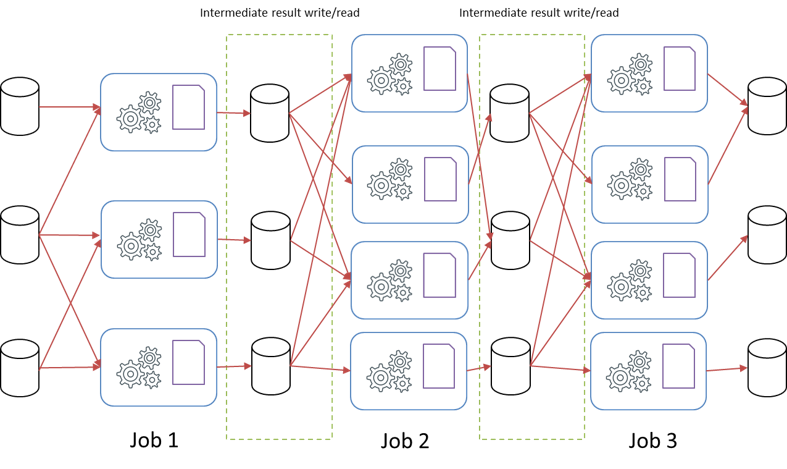
\includegraphics[width=32em]{./Figures/hadoop-high-io}
	\begin{figure}[htbp]
    \caption{High Input/Output behavior when iterative jobs performed on MapReduce}
    \label{fig:hadoop-high-io}
	\end{figure}
\end{center}
 This leads to a long execution time. Hence, it doesn't suit our requirements of supporting iterative operations as a pipeline and not a near-real-time responsive programming model. 
\subsubsection{Dryad and DryadLINQ}
Dryad\footnote{http://research.microsoft.com/en-us/projects/dryad/} is a general purpose framework for distributed, parallel-data applications created at Microsoft Research. Dryad, mainly focused on providing simplified programming model for parallel and distributed application development and their scalability, reliability and efficiency \cite{DRYAD}. A Dryad application consists \textit{vertices} that communicate to \textit{channels}, which eventually creates dataflow graph. Dryad supports executing multiple operations as a Directed Acyclic Graph (DAG) that eliminated the problems addressed by MapReduce. Further, Dryal also provided not only Map, Reduce, but also more features like sort, group. DryadLINQ\footnote{http://research.microsoft.com/en-us/projects/DryadLINQ/} is a powerful general purpose programming model provided by Dryad. DryadLINQ provides a simple declarative programming interface by supporting general-purpose imparative and declarative operations on data-sets within a traditional high-level programming language \cite{DryadLINQ} by utilizing Language-Integrated Query (LINQ) expressions. This enables flexible and efficient distributed in programming languages such as C\#, VB and F\#. Although, it is not available as an open source or commercialized solution, rather internally used in Microsoft. Dryad also inherits the performance penalty from MapReduce, as data must be reloaded from disk \cite{Spark}.
\subsubsection{Apache Spark and Resilient Distributed Dataset}
\label{sec:spark}

\textbf{In-memory cluster computing} 

Apache Spark\footnote{http://spark.apache.org/} is today's "de-facto" of big data, a general purpose distributed data processing framework, which is built to meet recent big data requirements such as iterative jobs and interactive analysis \cite{Spark}.  Spark sets a new computing paradigm called \textit{in-memory cluster computing} \cite{RDD} , using its main abstraction called \textit{resilient distributed dataset}, which holds a read-only representation of data object distributed across a set of machines (i.e. on Distributed Shared Memory (DSM)), that is fault tolerant \cite{RDD}. This eliminates the drawback of  having high I/O by not storing and loading back intermediate results of every iteration as depicted in Figure \ref{fig:in-memory-computing}.
 \begin{center}
	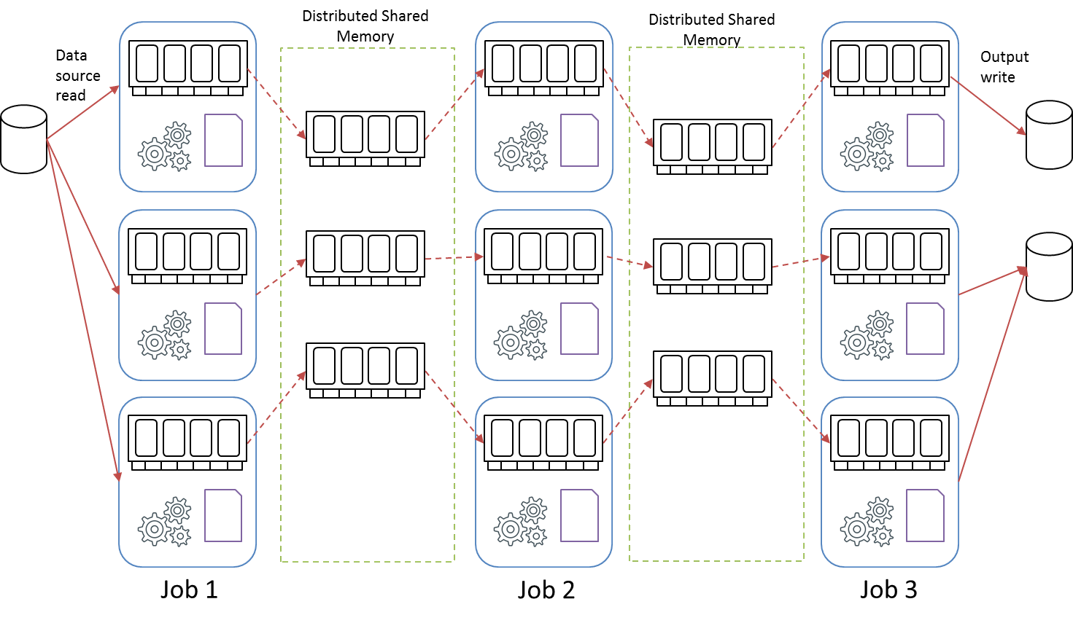
\includegraphics[width=32em]{./Figures/in-memory-computing}
	\begin{figure}[htbp]
    \caption{Behavior of in-memory-computing with iterative jobs}
    \label{fig:in-memory-computing}
	\end{figure}
\end{center}
Spark's another main aspect is parallel operations provided by spark, that can execute in parallel on different data partitions. Spark is claimed to be 10x - 100x faster than Hadoop in iterative applications \cite{Spark}\cite{RDD} \citep{clashoftitians}, by benefiting from Spark's programming model. Spark also provides distributed cache and shared variables to reuse computed resources that suits iterative computation. Spark also utilizes Hadoop's HDFS and YARN implementations. Spark is also considered as the open sourced implementation of research work done in Dryad. Spark also provides simplified language integration and functional programming syntax to write distributed computing applications \cite{Spark}\cite{Spark-improvements} and executes Spark jobs in DAG similar to DryadLINQ. 

The primary difference between Dryad and Spark is that Dryad cannot efficiently perform problems of iterative algorithms \cite{spark-vs-stratosphere}. In contrast to DryadLINQ, Spark lets RDDs to be persisted in memory across parallel operations. Further, Spark provides additional features like shared variables and cache which were not supported by Dryad \cite{Spark}.

\textbf{Spark's Strong Eco System}

Spark is one of the most widely used open source big data processing engine \cite{Spark-scalable}. Spark provides fully featured functional Application Programming Interface (API) in multiple languages Scala, Python, Java and R. In addition, Spark also evolved with providing underlying support for distributed processing of tabular data using Spark SQL \cite{SparkSQL}, graph data using GraphX \cite{GraphX}. Further, Spark also provides large scale machine learning libraries and support for stream and micro-batch processing. Figure \ref{fig:spark-prog-models} shows the main programming components provided by Spark eco system. 
 \begin{center}
	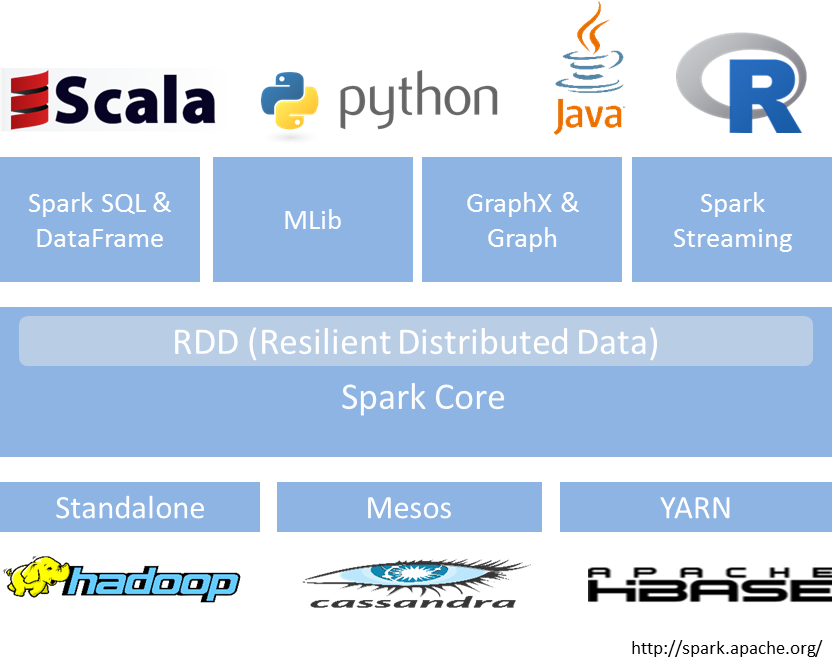
\includegraphics[width=32em]{./Figures/spark-programming-components}
	\begin{figure}[htbp]
    \caption{Programming components of Apache Spark Eco System}
    \label{fig:spark-prog-models}
	\end{figure}
\end{center}

\textbf{Lazy-evaluation of Spark Jobs} 

Moreover, RDD is an immutable distributed collection of objects. Making use of immutable object user can easily perform side-effect-free computation. Spark provides two types of operations that can be executed on RDD namely \textit{transformations} and \textit{actions}. \textit{Transformations} create a new RDD from previous one, whereas \textit{Actions} compute results based on a RDD and return it to driver program or store in external storage system (e.g. HDFS). Execution of a Spark job with multiple tasks are performed \textit{lazily}, such that the transformations are actually executed only when it reach an action. Until a pipeline reaches an action, the transformations are stored only as a meta-data \cite{learnspark}. When an action is reached Spark sees the whole chain of transformations, and compute the result needed. This provides a great level of optimization of jobs with pipeline of tasks, specially when large data is processed. 

\textbf{Scalable runtime architecture of Spark}

Spark uses master/slave architecture during distributed mode. It uses one central coordinator and many distributed workers to execute a given job. The central coordinator or master process is called \textit{Driver}. A driver communicates to large number of distributed workers which are called \textit{executors}. They compose a \textit{Spark application} which is launched on cluster of machines using an external service called \textit{cluster manager}. Spark works with cluster managers such Hadoop YARN, Apache Mesos and has its own standalone manager. 
\begin{center}
	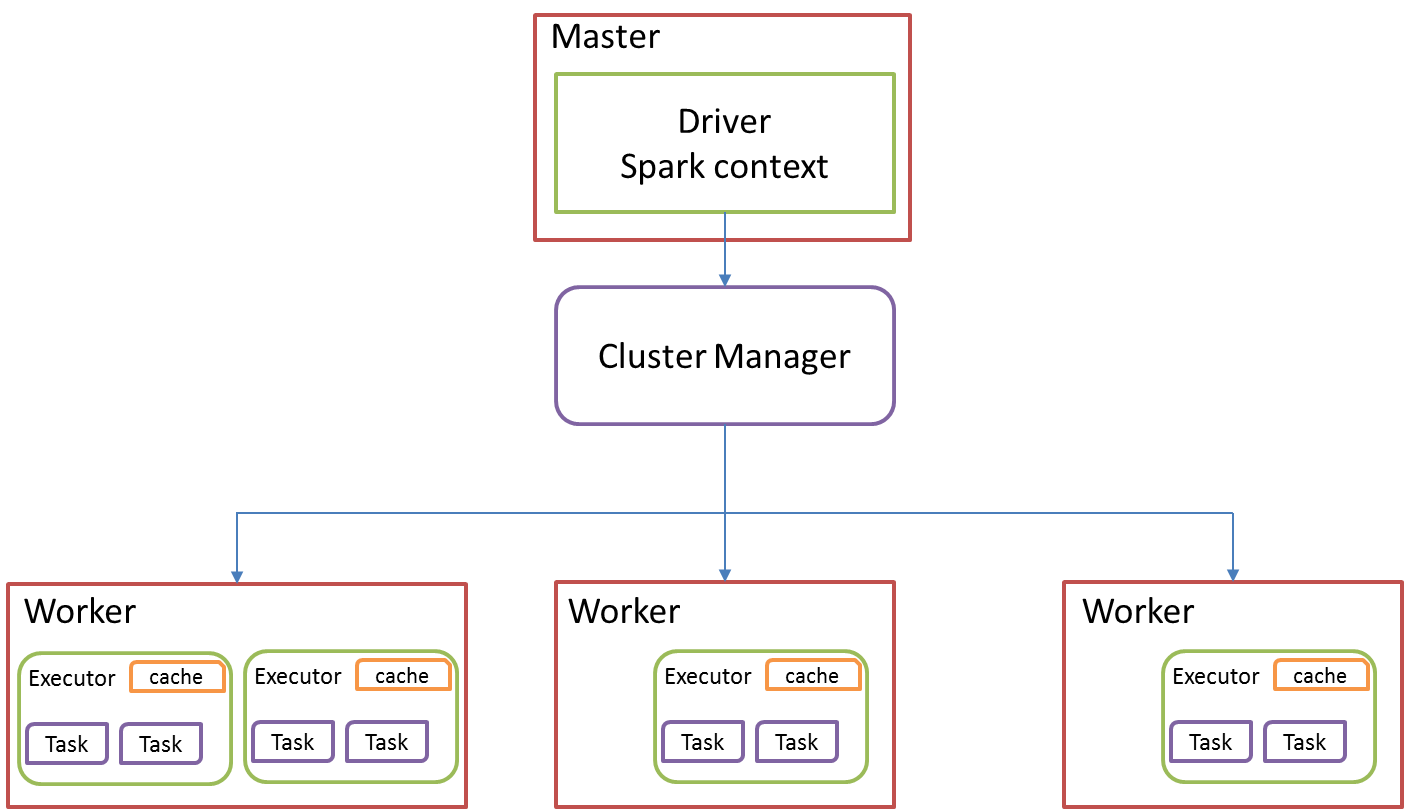
\includegraphics[width=28em]{./Figures/spark-master-slave}
	\begin{figure}[htbp]
    \caption{Spark's runtime architecture in distributed mode}
    \label{fig:spark-masterslave}
	\end{figure}
\end{center}
\textit{Driver} is the process which creates a SparkContext, creates RDD, converts user programs into spark\'s physical execution tasks, and creates logical representation of them in a DAG form and inform them to distributed workers. \textit{Executors} are the worker processes that performs individual tasks in a job. Executors are launched when a spark application is started and they typically run till the spark application stops unless there is a failure. Executors register themselves with driver process and receive and respond to driver according to the tasks given. Driver handles the rest.  Spark provides scripts to submit spark applications to cluster which is called \textit{spark-submit}. According to the configuration in spark-submit a spark cluster is launched. This lets the application to scale according to the cluster configurations mentioned in spark-submit. 

From these analysis, we can safely conclude that Apache Spark fits our purpose well better than other systems. Hence, we choose Apache Spark as our base platform and in-memory computing on RDD as our programming model to perform scalable, interactive and iterative open data cleaning.
\section{Summary}
After analyzing important requirements and solution fundamentals, we have noted that batch-processing is the correct ingesting method to do data cleaning on offline messy data. Secondly, in-memory computing and distributed data parallelizatoin from Apache Spark can be exploited to perform interactive, iterative data cleaning. 
% % Chapter 4

\chapter{Implementation} % Main chapter title
\label{Chapter4} % For referencing the chapter elsewhere, use \ref{Chapter4} 

\lhead{Chapter 4. \emph{Implementation}} % This is for the header on each page - perhaps a shortened title

%----------------------------------------------------------------------------------------
In this chapter,Implementation using the approaches and tools that are considered to enable the Scalable Open Data Transformation as a Service, following the results from Chapter \ref{Chapter3} are discussed in detail. Firstly, the important high level general design aspects that are considered described with the reasons behind the decisions. Important design level and implementation level requirements, best practices and guidelines that we followed are explained with example implementation approaches.  Further, specific aspects that were considered according to the research motivation (The DataGraft project) are also notified. 
\section{Solution Design}
We detail the system architecture design and important components of architecture that will be detailed later, which enables the Scalable Open Data Preparation as a Service. First, we focus on the high-level components and architecture that compose them together to meet our requirements. We also describe the facts that we considered during our design phase that enabled our solution. 
\subsection{High Level Architecture}
The design of our scalable open data preparation tool follows Component Based Software Engineering (CBSE) \cite{CBSE} aspects, inherited from motivational project DataGraft. We aim to design according to \textit{separation of concerns}, and with the help of Service oriented Architecture (SOA) techniques the individual components will be integrated. This ensures that the solution components to be reusable and loosely coupled. 

Recalling our requirements from Section \ref{sec:fundamentals}, We want to provide a "\textit{Solution as a Service}" that is interactive, incrementally builds the data preparation with iterative transformations with near-real-time responsive results and execute the transformation on provided input data. Provided that we focus on providing a simplified solution that can engage with marginal audience without requiring technical skills, we require an \textit{automated system} that can  internally handle complex process activities. 

Our solution will be a web-based solution, to provide collaborative transformation, availability and accessibility and user friendly solution. It will be integrated to DataGraft project via its interactive tool Grafterizer. Making use of AJAX\footnote{https://en.wikipedia.org/wiki/Ajax\_(programming)} programming, we provide an interactive and responsive data preparation service. Our solution has 4 main components, which are mentioned below:
\begin{enumerate}
\item \textbf{Grafterizer} : The interactive tool of DataGraft, that can interactively build data preparation pipeline. Grafterizer is responsible to provide interactive user interface to build data cleaning and RDF mapping,  render data cleaning results in real-time and provide interface to execute a completed data preparation. Grafterizer closely follows  user interaction and perform data transformation and rendering seamlessly. It implicitly generates data transformation pipeline using a Domain Specific Language (DSL) and request the back-end to execute the transformation pipeline. 
\item \textbf{Mem-cache} : Mem-cache is an intelligent caching system, that caches the results for each step in transformation pipeline. Mem-cache optimizes the whole process by cleverly inspecting every transformation request with available cache and responds the cached result if a cache-hit is found, or delegates the request to back-end to execute the transformation and caches the new results for corresponding request. This can significantly improve the performance of the system, by eliminating redundant requests. 
\item \textbf{Scalable-graftwerk} : Scalable-graftwerk is a \textit{Data Transformation Engine as a Service}, that executes the transformation pipeline sent from client program \textit{on-the-fly}. This provides RESTFul \cite{restful} APIs to execute scalable open data transformation pipeline. This encapsulates the complex integration with scalable data preparation tool by wrapping the scalable transformation APIs with a DSL. The transformation pipelines generated and sent from client program are sent to Scalable-graftwerk using provided RESTFul APIs. Scalable-graftwerk's transformation execution engine executes the transformation pipeline sent with the request and replies the results as a HTTPResponse.  
\item \textbf{Sparker} : Sparker is the scalable open data transformation tool what will perform the actual job. Sparker comlies to the tools and requirements mentioned in Section \ref{sec:fundamentals} and Chapter \ref{Chapter3}. Sparker is wrapped using domain specific APIs by Scalable-graftwerk and exposed as a RESTFul service to users. 
\end{enumerate}
According to the discussions in Chapter \ref{Chapter3}, the solution should be scalable that can be scale-in or scale-out on a distributed environment. Figure \ref{fig:architecture} depicts how the components discussed above are composed together on cluster of distributed machines. 
\begin{center}
	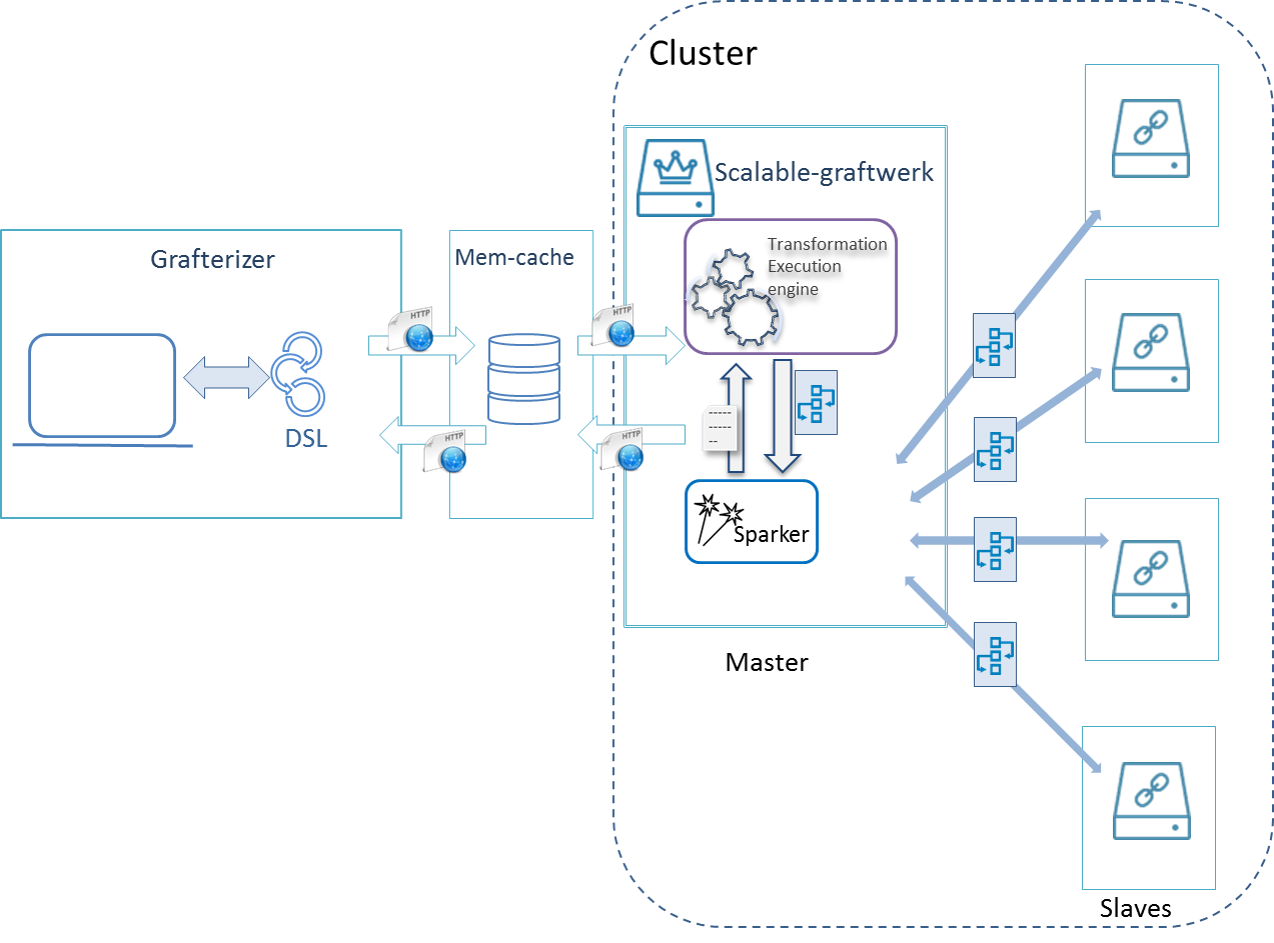
\includegraphics[width=38em]{./Figures/architecture}
	\begin{figure}[htbp]
    \caption{Scalable Data Transformation as a Service Architecture}
    \label{fig:architecture}
	\end{figure}
\end{center}
\subsection{Process Work-flow Diagram}
Figure \ref{fig:workflow} illustrates how a data preparation process is handled by our solution. User initially loads input file using Grafterizer. A user is given an option to decide whether to perform the interactive transformation on a sample of data or not. Open data can range from small to large volumes of data. Having said that, the option to create a sample allows user to decide according to the size of raw-data. 
\begin{center}
	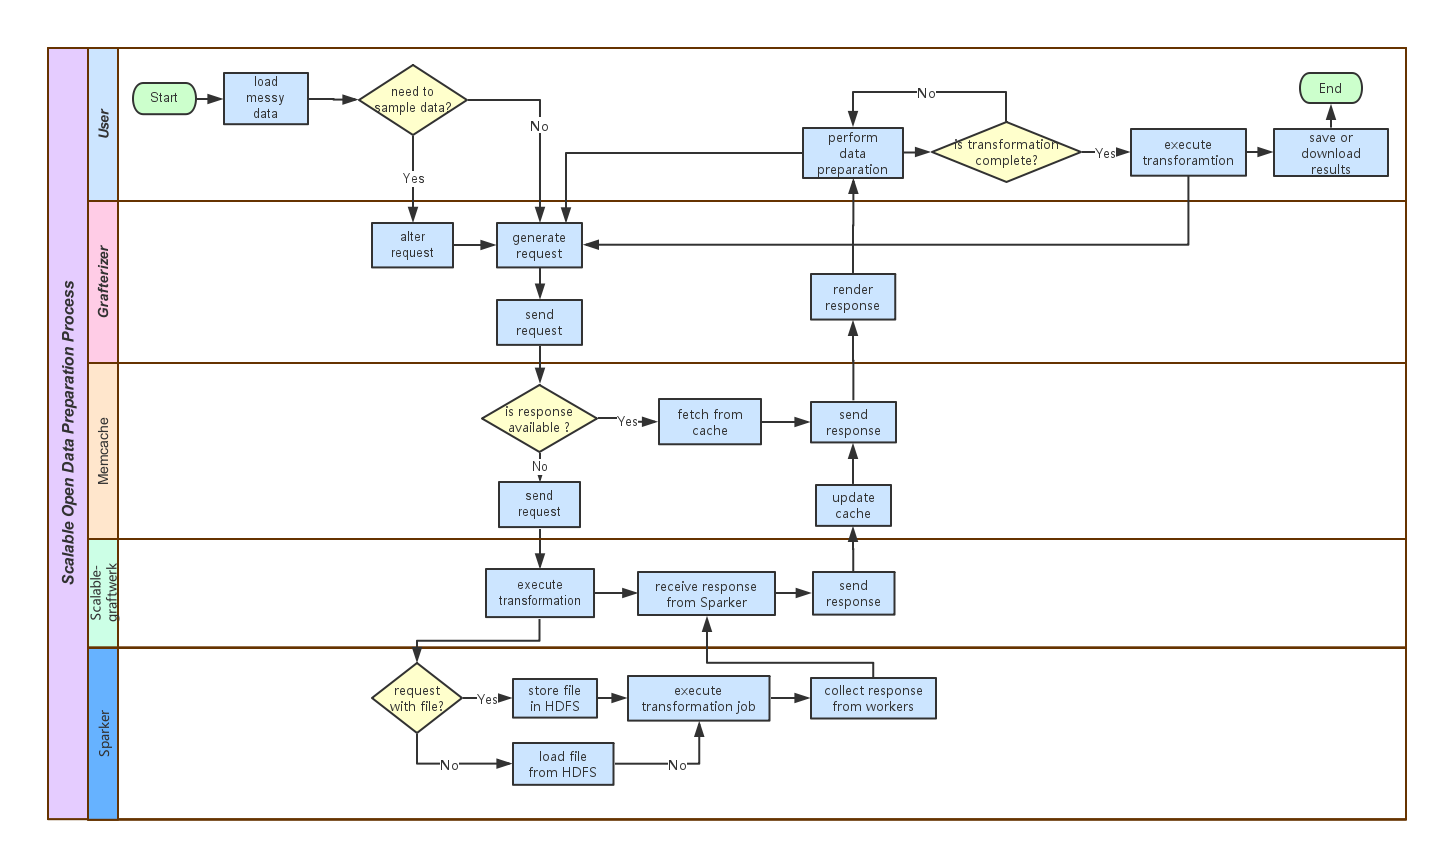
\includegraphics[width=55em, angle=90]{./Figures/work-flow}
	\begin{figure}[htbp]
    \caption{Optimized data preparation work-flow of large data}
    \label{fig:workflow}
	\end{figure}
\end{center}
If the data processed exceeds allocated quota of interactive transformation data size, it will be sampled by the system and initial file and sample files stored by back-end system. Then user can perform incremental, interactive transformation on data. When user is satisfied with transformation, user can execute the transformation on the whole data which is already stored at the back-end. Once the data transformation is performed, back-end will remove stale data.

\section{Solution components}
In this section we describe the basic components that are used to come up with the final solution engine, with supporting reasons for design decisions. 

\subsection{Sparker}
\label{sec:sparker}
The main challenge to be solved is to provide a scalable open data preparation solution using the techniques and technologies selected in Chapter \ref{Chapter4}. Provided that we follow \textit{separation of concerns}, we decided to implement the distributed open data preparation operations including data cleaning and linked data creation in a separate project called \textit{Sparker}. 
\subsubsection{Design level requirements}
\label{designreq}
We further analyzed the important requirement that need to be considered during our implementation and design level. Specifically, we require the data preparation tool to support,
\begin{enumerate}
\item Easily integrated with dynamic execution engine : The end-user solution is expected to be interactive and user friendly. This requires the data preparation operations to be built dynamically and executed on demand. Thus, it requires to provide Application Programming Interface (API) driven component.
\item Pattern oriented APIs : The data preparation operations are need to be provided as independent APIs that can be easily executed as pipeline of operations. To have intuitive pipeline creation of data preparation operations, all APIs should follow a pattern that can ensure seamless pipeline generation.
\begin{itemize}
\item \textit{\textbf{Chain-of-responsibility (COR) pattern}} : We need a pattern that can help to create pipeline of APIs provided. As we discussed earlier, data preparation will be performed iteratively and incrementally. Hence, the pipeline should reflect on incremental updates of data preparation.COR pattern a design pattern that has a parent command followed by series of processing commands. Each command has designated logic and input/output to handle and the rest are passed to the next processing command. This mechanism is also very helpful when adding an additional processing command at the end of the chain. The end result will contain the result of execution of all operations. 

For example if an API to select range of columns is given as take-columns(to,from) and drop-columns(to,from) to drop data, execution of take-columns(1,2) on data with columns A, B, C, D should result with a data with columns A, B, while if execution of drop-columns(1,2) then take-columns(1,2) should result in data with C, D, not with A,B or any other. 
\item Following the COR pattern and by adopting Builder pattern, we require the APIs to take same type of basic input parameter and should result in same type of output such that the pipeline can be easily created. 
\end{itemize}
\item Functional Separation between API : There should be clear separation between each API given, such that the execution of that operation does not provide results with side-effects at any of the combination of data preparation pipeline. Each API should be clearly broke down into specific behavior of the operation. (e.g. merging two columns should be separated from renaming merged column name). CBSE aspects can be considered during API level design too.
\end{enumerate}
\subsubsection{Functional requirements}
The next step is to identify the data preparation operations that need to be implemented. We gathered requirements from the motivational project and other related systems to provide a complete solution. Initially, we plan to implement data cleaning operations required by DataGraft and sample POC operation to create an RDF using simple mapping. However, we require the basic design should be able to evolve continuously according to future open data preparation needs. We conducted a feasibility analysis to see how can DataFrame APIs re-purposed to meet our needs. 
\subsubsection{Tools and Approaches}
An implicit requirement of our solution is to have a flexible low-level data abstraction that should be scalable such that it can be easily convertible to tabular data or to graph-based model. Referring to the systems in Section \ref{sec:relatedwork}, it can be clearly seen that the large-scale applications are focused on individual solution. One of the main impediment to evolve to fit open data requirements can be, lack of an interchangeable data abstraction. It is must our programming model and data abstraction meet this requirement. To confirm this requirement, we analyzed Spark's core components in detail. 
\begin{itemize}
\item \textbf{DataFrame} 

DataFrame is a collection of distributed data grouped into named columns (i.e. RDD with schema), that can perform relational operations on both RDD built from external sources and built-in collections \cite{SparkSQL}. DataFrame object can be easily created from RDD or from external resources as well as converted to RDD easily. It provides API for basic relational operations that can execute in parallel on distributed data.  Pipelines of operations can benefit from being lazily executed as mentioned in Section \ref{sec:spark}. Further, Figure \ref{fig:rdd-vs-dataframe} from an evaluation study from Databricks \cite{databricks-dataframe}(the designated paid maintainer of Spark), says that DataFrame is significantly faster than RDD when aggregation operations are performed.
\begin{center}
	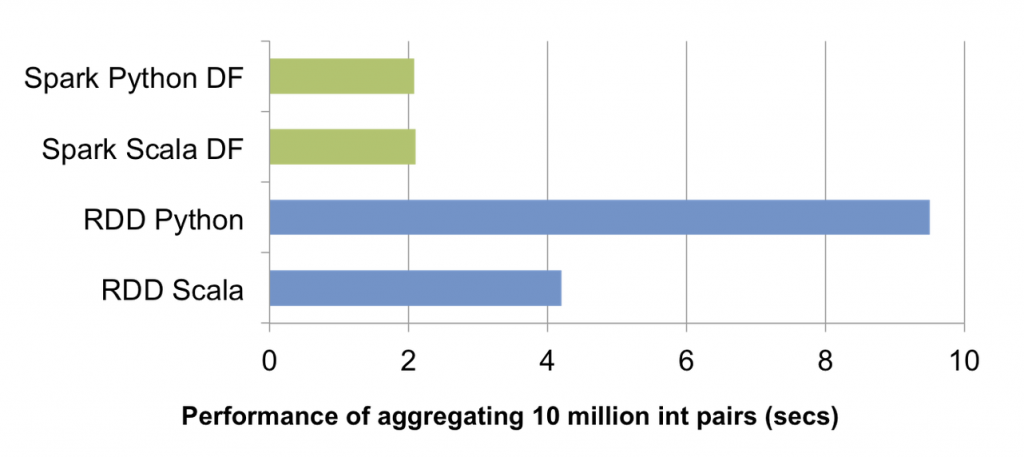
\includegraphics[width=38em]{./Figures/rdd-vs-dataframe}
	\begin{figure}[htbp]
    \caption{Programming components of Apache Spark Eco System \cite{databricks-dataframe} }
    \label{fig:rdd-vs-dataframe}
	\end{figure}
\end{center}
By utilizing lazy evaluation of ETL operations, Spark SQL can perform relational optimization \cite{SparkSQL} which satisfies our requirement (R6). Lastly, Spark SQL extends a novel optimizer called Catalyst. Catalyst supports both rule based and cost-based optimization \cite{SparkSQL}. This explains that DataFrame and Spark SQL can be exploited to represent messy data as tabular data and perform data cleaning, with internal relational optimization and query optimization.
\item \textbf{GraphX's Graph }

GraphX is a distributed graph computation model, that unifies graph-parallel and data-parallel computation \cite{GraphX}. This unified abstraction enables the same data to be represented as graph and tables without data movement or duplication. GraphX uses RDDs as the foundation for distributed collections and graphs. The property graph data model in GraphX was adopted from RDF graph \cite{RDFinGraphX}. The property graph corresponding to an RDF graph contains the predicates as edge properties and the subjects and objects as vertex properties. Thus, it is a strong base to create distributed graphs using RDD. 
\end{itemize}
Figure \ref{fig:dataabstraction} shows how the data abstractions discussed above can create an interchangeable data abstraction for our open data preparation system. The abstraction mentions the interchangeability of DataFrame to/from RDD and interchangeability of Graph to/from RDD. This can result in a flexible data abstraction that can solve our requirement.
\begin{center}
	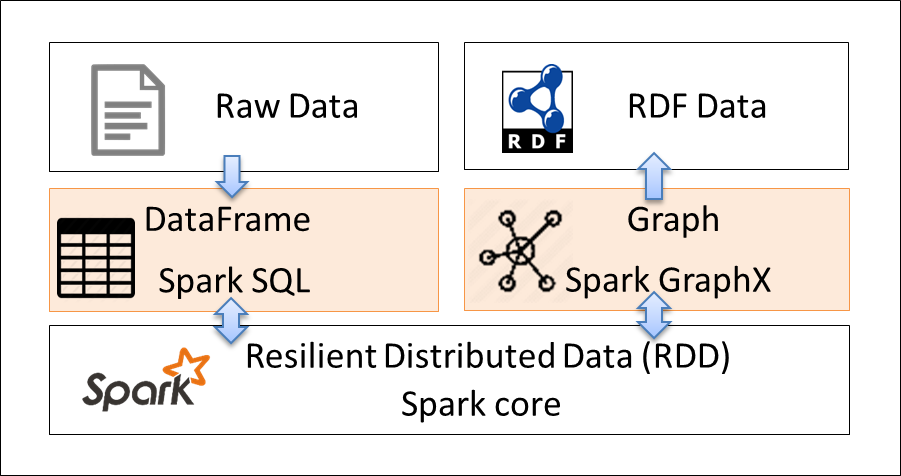
\includegraphics[width=35em, height=15em]{./Figures/data-abstraction-prog-model}
	\begin{figure}[htbp]
    \caption{Inter-changeable distributed data abstraction}
    \label{fig:dataabstraction}
	\end{figure}
\end{center}
Follwing the discussion in Section \ref{sec:sparker}, we designed our system as follows. Figure \ref{fig:package-diagram} shows the use case package diagram\footnote{http://agilemodeling.com/style/packageDiagram.htm} of Sparker. It shows that \textit{sparker.tabular} package, that is allocated to perform data cleaning activities on tabular data uses \textit{spark.sql} libraries including \textit{DataFrame} and \textit{sparker.rdf} package which is responsible for RDF creation uses  \textit{spark.graph} libraries to create graphs that uses \textit{Triplets}. Also there are internal supporting sub-packages named \textit{util} implemented to support data cleaning operations in DataGraft.
\begin{center}
	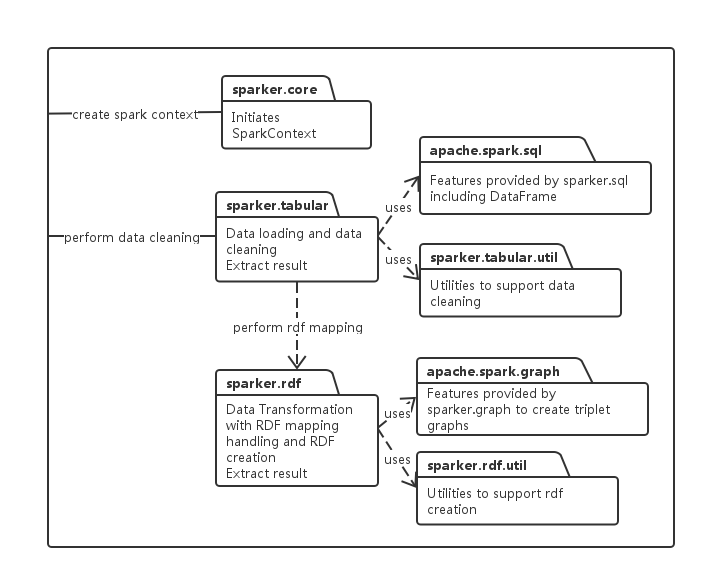
\includegraphics[width=35em, height=23em]{./Figures/Class_Diagram}
	\begin{figure}[htbp]
    \caption{Use case package diagram of Sparker}
    \label{fig:package-diagram}
	\end{figure}
\end{center}
\subsubsection{Choice of language and versions}
We decided to do the implementation using Scala\footnote{http://www.scala-lang.org/} among the languages Spark supports such as Scala, Python, Java and R. Scala is a current hype of Hybrid Languages that have insights of both Functional Programming (FP) and Object-Oriented-Programming (OOP) \cite{scala-book}. Scala runs on Java Virtual Machine (JVM) and interoperable with other JVM compatible programming languages. Hence, Sparker also can use any utilities implemented in JVM languages as well as can be used in all JVM languages. Moreover, Spark's initial implementations were using Scala, which ensures of strong and active community support and availability of feature implementations, extensions and plugins etc. We chose Scala 2.10.6 and Spark 1.6.0 versions for our implementation, as there were the latest stable releases. 
\subsubsection{Distributed data cleaning operations}
 The final challenge to solve in Sparker was to implement data preparations in distributed-data-parallel manner. We first focus on the implementation of data cleaning operations on tabular data. To make it clear, we introduce some basic explanations of how DataFrame behaves in distributed context and implementation on top of DataFrame should be approached. 
 
 \textbf{Spark and DataFrame Basics}
 
 Spark executes its tasks on RDD. Each RDD is split into number of partitions that may reside on different nodes of cluster. Number of partitions of RDD defines the basic level of distributed parallelism we can have. DataFrame extends RDD, which is also partitioned and located in different nodes of a cluster. Performing operations on a "distributed-table" is challenging. Following facts are important to be considered when data preparation functions are implemented.
\begin{itemize}
\item \textbf{Distribution of schema} : DataFrames are created with a schema that represents the structure of data, which is distributed to all partitions over distributed nodes. When the schema of the data is modified, the data need to be redistributed with updated schema, as all nodes should hold identical and up-to-date schema. When an operation is executed, every executor reads the schema and perform the operation based on the schema (if it depends on schema). 
\item \textbf{Distinction of transformations and actions of data cleaning operations} : Column level operations such as \textit{filter data, drop column} are easily performed on DataFrame, as they are usually types of \textit{transformations}. However, when \textit{actions} are performed on data (e.g. group and aggregate) then the driver needs to load the data from all partitions to a single memory and store them in external storage or re-partition the new RDD. Execution of \textit{actions} involve\textit{ data shuffling} from nodes, which is expensive than execution of \textit{transformation}. 
\item \textbf{Number of partitions} : As mentioned earlier number of partitions are the crutch of parallelization we can get during an execution. Ideally, Spark calculates the number of partitions according to the SparkContext and the data being processed. However, the DataFrame can be re-partitioned.  Having less number of partitions may result in less parallelism as well as having large number of partitions may result in huge overhead during data shuffling. 
\begin{itemize}
\item \textit{A Rule of Thumb} : A function should be always implemented with minimal data shuffling and auto-partitioning if the size data being process is subject to change, unless otherwise it is required. An implementation should try to consist more transformations or less frequent actions. 
\end{itemize}
\item \textbf{Memory allocation of Driver according the data being processed} : When data is shuffled from all nodes, the parent node should be able to hold the whole data in single memory without running out-of-memory problems. Hence, it is important to have a rough estimation of maximum size of data being processed and allocate Driver memory accordingly. 
\item \textbf{Addition of new data should be identically partitioned with primary data} :  Having said that, the RDD/DataFrame is partitioned, new data that need to added should also be identically partitioned. By \textit{identical} we mean equal number of partitions and equal number rows of each partition. The data that needs to be added should be partitioned in a way that it has one-to-one mapping to the rows that are in each partitions. 
\item \textbf{Rows that comply with schema} : Each row values of the table should comply with the schema, based on number of columns and structure of column and types of column.
\end{itemize}
Adhering to the above notes we implemented data cleaning functions on top of DataFrame API. 
\subsubsection{Implementation of Data Cleaning operations}
To explain how we carried out our implementation 1) adhering to the notes mentioned above, 2) utilizing the functional programming aspects 2) utilizing object-oriented programming aspects, we discuss few examples below. 
\begin{enumerate}
\item \textbf{Make dataset with a range of columns }

This operation doesn't involve in data shuffling as it is completely depend on columns that can be identically performed on all partitions. Using Scala APIs and DataFrame APIs we select a subset of column list using given range, perform a \textit{select} operation like \textit{SQL Select} to create new DataFrame. 
\begin{center}
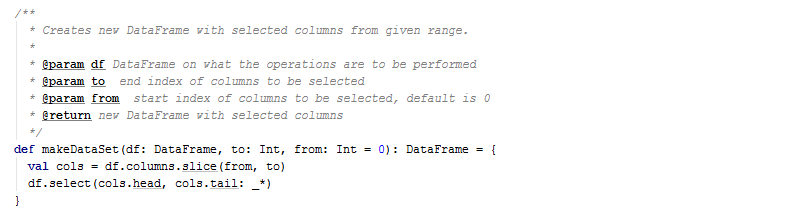
\includegraphics[width=38em]{./Figures/take-columns}
\begin{figure}[htbp]
\caption{Implementation of making dataset with range of columns}
\label{fig:take-columns}
\end{figure}
\end{center}
It can be clearly seen that the API provided is very intuitive and straight forward to use by the end user. 
\item \textbf{Merge columns}

When we want to merge a set of columns with a separator as shown in Figure \ref{fig:merge-columns-exp}, we need to create a new column i.e. it alters the schema. The below example explains how DataFrame API can be exploited when a new column is added. 
\begin{center}
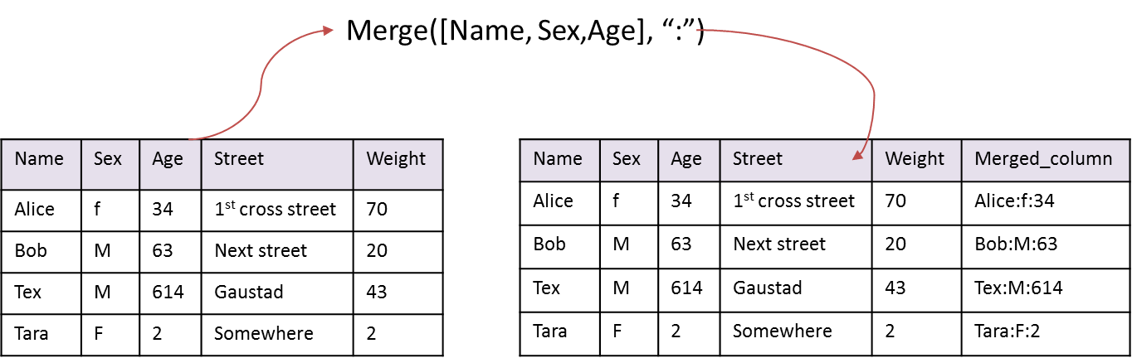
\includegraphics[width=30em]{./Figures/merge-col-exp}
\begin{figure}[htbp]
\caption{Explanation of merge columns}
\label{fig:merge-columns-exp}
\end{figure}
\end{center}
\begin{center}
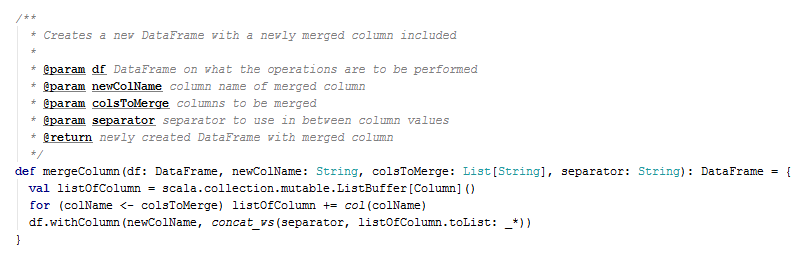
\includegraphics[width=38em]{./Figures/mergecolumn}
\begin{figure}[htbp]
\caption{Implementation of merging set of columns}
\label{fig:merge-columns}
\end{figure}
\end{center}
 The \textit{withColumn} API from DataFrame, handles the schema verification and if the column name provided is not available as a column already, it creates new schema with additional column with provided name (\textit{newColName}) and sends to all partitions. The \textit{concat-ws} is an implicit function provided by \textit{spark.sql} which takes arbitrary number of columns and merge them with provided separator. Every executor who sees the \textit{withColumn} function takes the \textit{newColName} from schema and sets the value from \textit{concat-ws} on right position. We must note that all these operations are performed based on columns, so data shuffle is performed. 
\item \textbf{Add row id }

When user wants to add a column with row id (row number), these row numbers nor a column to hold row numbers are part of the partitions already. This operation needs to change the schema as well as the partitions to add new data. Further the additional data need to be one-to-one mapped with existing partition data. As easy way to add incremental ids can be done by \textit{zipWithIndex} API provided by RDD.This operation creates the partitions of RDD with incremental index that is mapped to each row in every partition, preserving the order of rows.   
\begin{center}
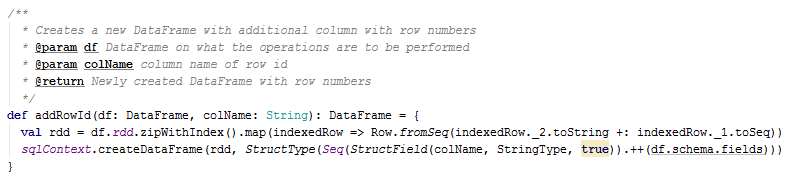
\includegraphics[width=38em]{./Figures/add-row-id}
\begin{figure}[htbp]
\caption{Implementation of adding a column with row id}
\label{fig:add-row-number}
\end{figure}
\end{center}
Making use of \textit{Map} operation, we create new Row with mapped index for each row. Then a new DataFrame is created using newly created RDD and newly created Schema which is called \textit{StructType} that has an additional column (\textit{StructField}).
This lets us to realize the level of technical and domain related abstraction provided by the implemented API.
\item \textbf{Melt data-set}

Reshaping\footnote{http://www.ats.ucla.edu/stat/stata/modules/reshapel.htm} data-set is an important requirement from data preparation sector. Reshaping data-set a powerful functionality that reshape the data according to user requirement. It is mostly categorized as \textit{wide-to-long} and \textit{long-to-wide}. We will see the implementation of a powerful reshape operation called \textit{\textbf{melt}}. Melt is a wide-to-long transpose operation of a data-set. 
\begin{center}
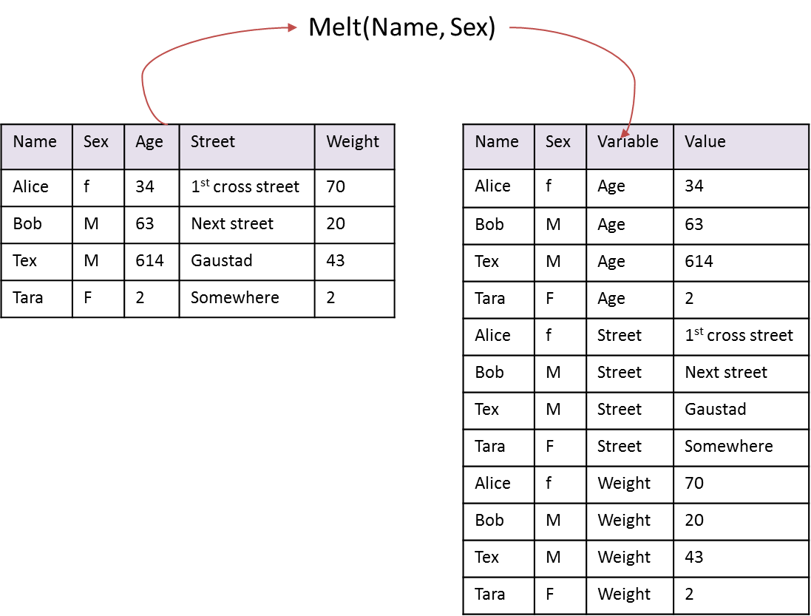
\includegraphics[width=30em]{./Figures/melt}
\begin{figure}[htbp]
\caption{Explanation of melt operation}
\label{fig:melt-exp}
\end{figure}
\end{center}
Melt operation is a very complex and expensive operation to perform. As reshaping data is not very common, we will first explain the behavior of \textit{melt} operation.Figure \ref{fig:melt-exp} depicts how a melt operation will result. Melt operation is performed to extract data that are included in column names. 
\begin{center}
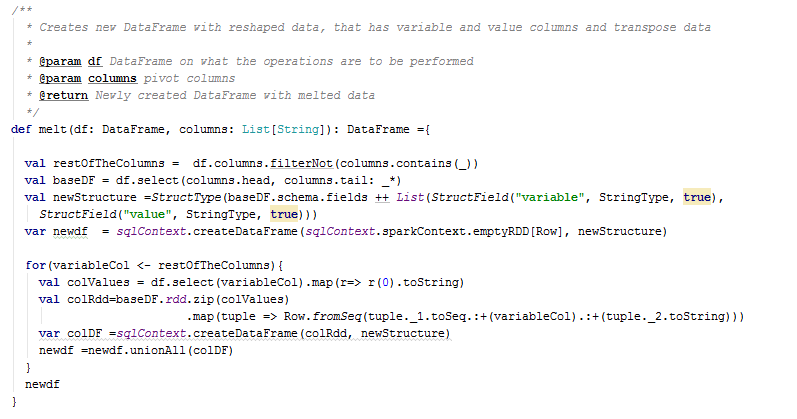
\includegraphics[width=38em]{./Figures/melt-impl}
\begin{figure}[htbp]
\caption{Implementation of melt operation}
\label{fig:melt-impl}
\end{figure}
\end{center}
To implement this functionality, we need to create new DataFrame with given pivot columns, create a schema with additional columns, then create \textit{Row}s for each columns with corresponding column name and value and perform a \textit{union} operation to merge these two DataFrames together, per column. 
\end{enumerate}
These examples illustrates that APIs eliminates the technical and domain related requirements a data-worker would need, and by providing simple, intuitive and schema-independent APIs that comply with the design requirements we discussed in Section \ref{designreq}. 
Table \ref{fig:features} shows the functions implemented by Sparker and brief description of the functions. 
\begin{center}
	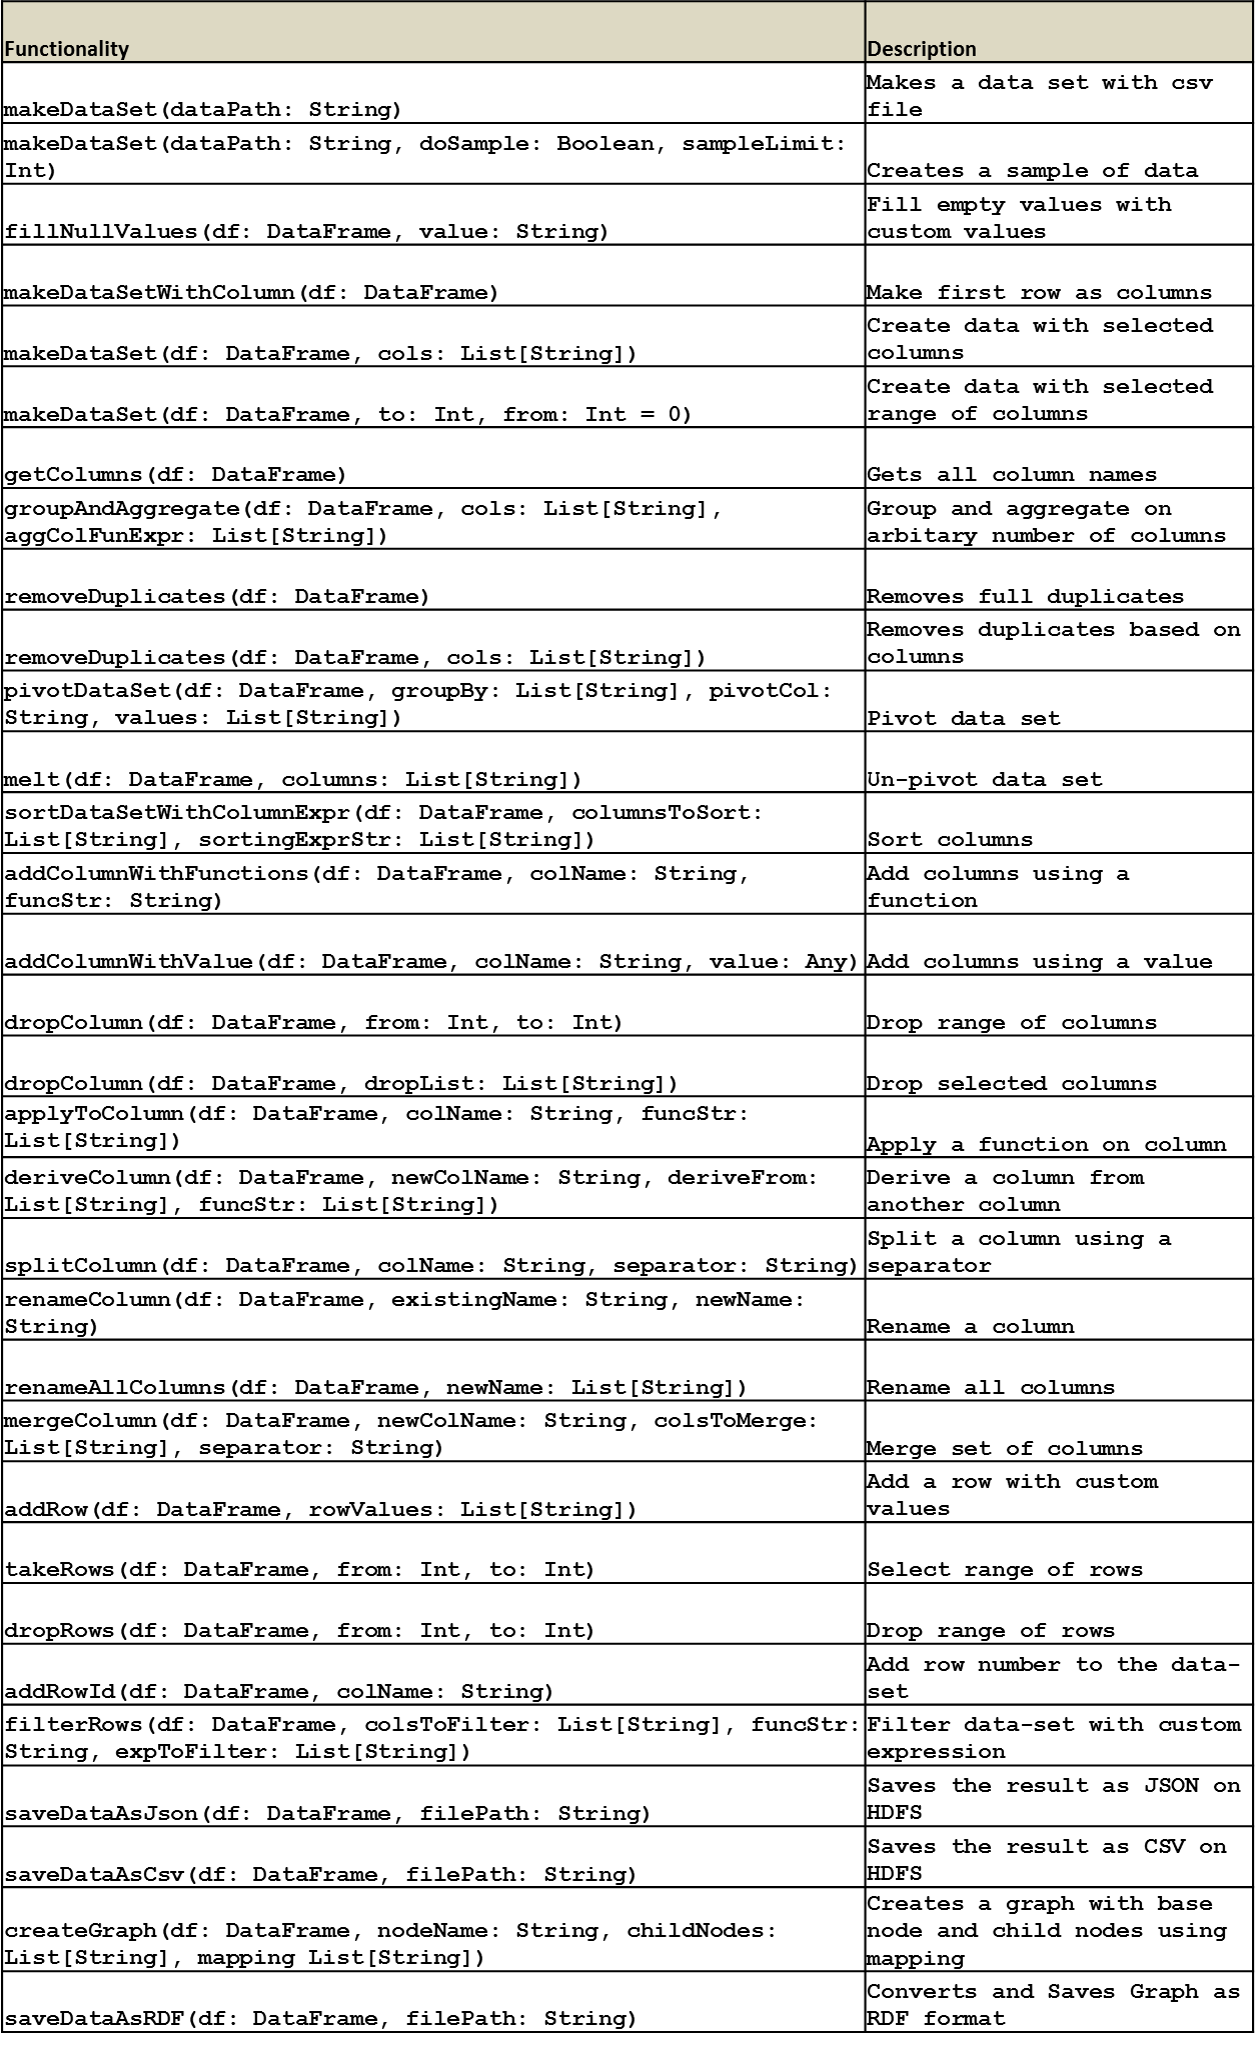
\includegraphics[width=35em]{./Figures/Picture2}
	\begin{table}[htbp]
    \caption{Table of Functions implemented in Sparker}
    \label{fig:features}
	\end{table}
\end{center}
\subsubsection{Implementation of RDF generation}
Generation of RDF from uncleaned data is our ultimate goal. RDF data of a tabular data can be generated by performing RDF mapping on tabular data. We can create a base node using a column or predefined literal. We currently, support simple RDF mappings, where a parent node is mapped with a child node using a property that explains the relationship between them. This results in specifying two columns of table and mapping information for each mapping ( e.g. Column "personID" can be mapped to column "name" with a mapping of foaf:name, i.e name property from foaf (Friend of a friend) vocabulary).  We create vertices of both specified columns, which contains unique VertexID as required by Spark graph for each row. Then we create an Edge that has (parentVertexId, childVertexId, mapping) for each record for each record. This results in a graph of \textit{Triplets}. Likewise, we perform this two operations for each mapping specified in a graph. Once the mapping is finalized,  we generate RDF in the form of N-triple, by concatenating values in each triplet of given graph. 

\subsection{Scalable-graftwerk}
Scalable-graftwerk is a service that provides dynamic transformation execution engine that executes a DSL and also provides an adapter of Sparker. We will discuss, the important features provided by Scalable-graftwerk and how it enables our solution to be interactive.
\subsubsection{Functional requirements}
\label{engine-req}
The important requirements to solve in Scalable-graftwerk are :
\begin{itemize}
\item \textbf{An environment with a dynamic language} : Data cleaning transformations are interactively created from client side. They should be built using a dynamically typed language also called as \textit{dynamic language }. A dynamic language is a programming language that just not gets compiled and run, but also can be added, changed functions at run-time and evaluated at run-time). 
\item \textbf{Dynamic execution engine of transformation} :  Each stage in a transformation pipeline should be evaluated dynamically during the interaction. Transformation pipelines are essentially programs or meta-data that needs to be dynamically executed. An execution engine should be created to evaluate the generated pipeline on-the-fly to provide response immediately.
\item \textbf{Dynamic APIs that wraps open data preparation functions} : Provided that we have an execution engine that can execute programs of a dynamically typed language, since we are using Sparker for scalable open data preparation, those data preparation features mentioned in Figure \ref{fig:features} must be adapted using the selected dynamic language, such that it can be used to create  transformation pipeline and executed by execution engine.
\item \textbf{RESTFul APIs} :  Lastly, our goal is to provide Scalable open data transformations as a Service. The requirements discussed above should be exposed as Web Service APIs that can be integrated with external systems. We chose to use RESTFul APIs adhering to the system designs of DataGraft. 
\end{itemize}
\subsubsection{Tools and Approaches}

\textbf{Clojure}

Referring to above requirements, we need a dynamic language to perform interactive execution of transformation pipelines. We used Clojure \cite{clojure} a functional programming language and a dialect of LISP\cite{lisp} programming language (a dynamic high-level-language). Clojure inherits  and \textit{dynamic typing} and fully \textit{parenthesized prefix notation} (i.e. a programming logic is mentioned using parenthesis having a function to evaluate and related parameters within the parenthesis e.g. \textit{\textbf{(add 1 2)}}) from LISP. Clojure runs on JVM and supports concurrent programming. Specially, Clojure provides \textit{\textbf{macros}}, which is a language construct in Clojure that can easily extend the language at compile time. Since Clojure is a dynamic language, type annotations are not required for code to run. Moreover, Taking advantage of  interoperability of JVM languages, Clojure can be easily integrated with other JVM languages. Since Clojure is a dynamically typed language that can run on JVM whereas Sparker is implemented using Scala which is also another JVM based language, the choice of Clojure fits our context well, than other dynamic languages such as Ruby, PHP, Lua and Perl. 

\textbf{Ring Server and Compojure Routes}

To provide a RESTFul service, We need a web server (A computer system that can process requests via Hypertext Transfer Protocol (HTTP), the basic network protocol used on the World Wide Web) that can process Web Services. We implemented our RESTFul Web Services using open sourced libraries including Ring\footnote{https://github.com/ring-clojure/ring} and Compojure\footnote{https://github.com/weavejester/compojure}. Ring is a Clojure library that provides abstractions of HTTP into simple and unified APIs. Ring allows a web application to be a collection of small independent modules. Routes in Ring are small modules that can compose a Ring Application. Compojure is a routing library for Ring, which provided simple APIs as macros\footnote{http://clojure.org/reference/macros}, that can be simply implemented as RESTFul Services. We chose Ring and Compojure as there were the state-of-the-art implementations of our requirements and widely used by Clojure community. 
\subsubsection{Sparker's Adapter in Clojure}
We need a \textit{dynamically typed} version of Sparker's functions. Following \textit{adapter design pattern} , we implemented an adapter that wraps Sparker's functions implemented as Scala APIs into equivalent Clojure functions. 
\begin{center}
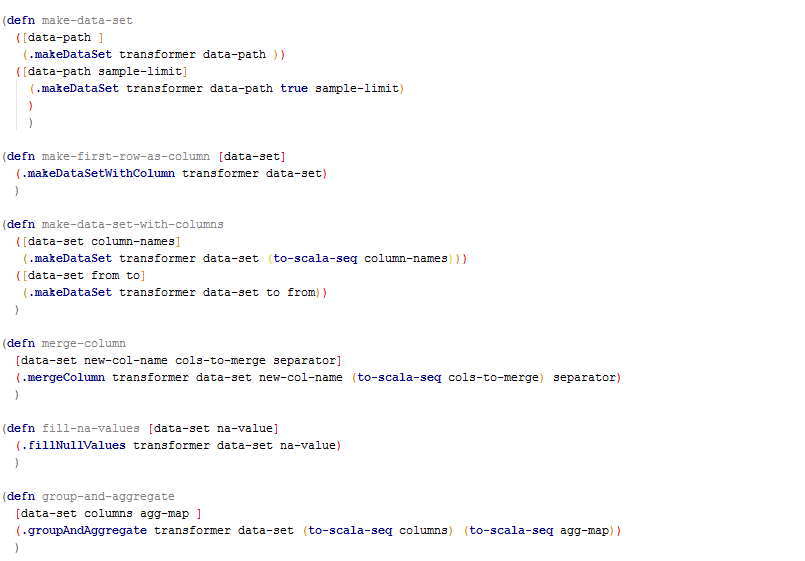
\includegraphics[width=36em]{./Figures/wrapper}
\begin{figure}[htbp]
\caption{Part of Sparker's adapter in Clojure}
\label{fig:wrapper}
\end{figure}
\end{center}
Figure \ref{fig:wrapper} shows the adapter of Sparker's functions in Clojure. A sample data transformation pipeline is shown in Figure \ref{fig:sample-pipeline} that creates a data-set with columns from first-row, then selects columns ranging from 0 to 15 and, then select specific columns by column names and lastly removes duplicates in groups based on provided set of columns. This example proves that the design requirements considered in Section \ref{designreq} have resulted in simple and easy creation of transformation pipeline. 
\begin{center}
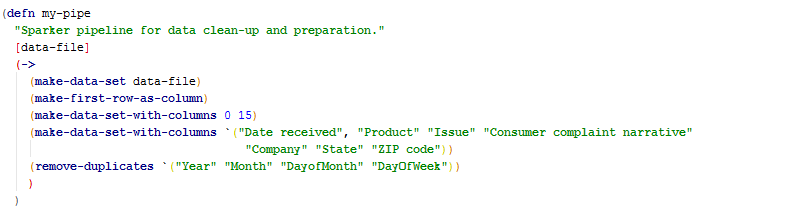
\includegraphics[width=36em]{./Figures/sample-pipeline}
\begin{figure}[htbp]
\caption{Sample pipeline using DSL of Scalable-graftwerk}
\label{fig:sample-pipeline}
\end{figure}
\end{center}
Clojure's thread first macro\footnote{https://yobriefca.se/blog/2014/05/19/the-weird-and-wonderful-characters-of-clojure/} take an initial value and thread this value through a number of forms. By passing output from previous command to following command this ensures that data pipeline processed for given input. 
\subsubsection{Scalable Data Transformation as a Service}
We adopted an open sourced implementation called Graftwerk\footnote{https://github.com/Swirrl/graftwerk}, which can perform similar tasks mentioned in Section \ref{engine-req}. Graftwerk has an in-built sandbox which securely execute arbitrary Clojure codes. Sandboxes are created with a secured execution context and can be configured to avoid execution of codes with security threads. Even though having a sandbox in a dynamic execution engine provides security, such sandbox with restricted context prevented us from executing Spark related code. Thus, we implemented an execution engine using Clojure's core library that can execute only the DSL defined in Scalable-graftwerk. Scalable-graftwerk's dynamic execution engine and scalable data transformation features can be accessed by external systems using provided RESTFul API.  Those Web Service APIs provided by Scalable-graftwerk eliminates execution and integration complexity of Sparker functions. 
Sample API implementation using routes and how such API can be used using a RESTFul client is shown in Figure \ref{fig:sample-route} 
\begin{center}
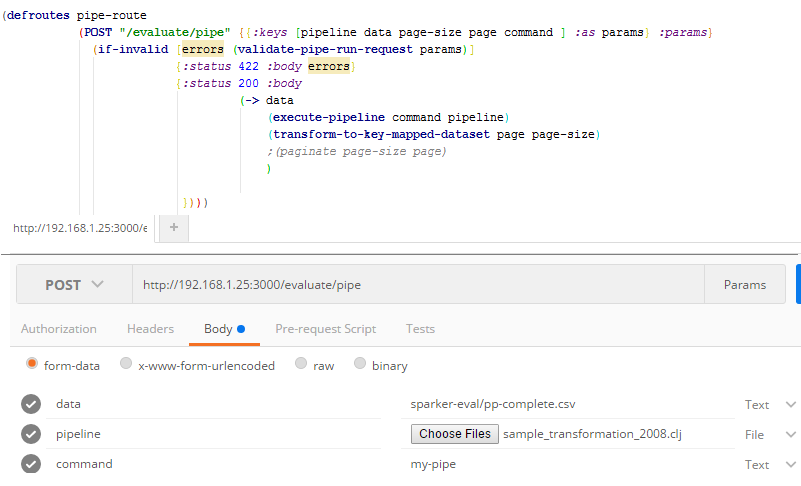
\includegraphics[width=36em]{./Figures/sample-route}
\begin{figure}[htbp]
\caption{RESTFul API of transformation engine and Execution of a sample transformation}
\label{fig:sample-route}
\end{figure}
\end{center}
\subsection{Grafterizer}
Grafterizer is the the interactive data transformation tool of DataGraft. Grafterizer has user friendly, spreadsheet like interface to display tabular data and user interfaces that provide easy means to build transformation pipeline. Once the data is cleaned, user can create RDF mapping using Grafterizer's RDF Mapping interface. During the data preparation process, Grafterizer automatically builds corresponding transformation pipeline scripts, creates and sends HTTPRequest to given RESTFul APIs. Once the response is received, using the response headers Grafterizer renders data in tabular format. 

\subsubsection{Functional requirements}
Grafterizer has a code generator, that can generate transformation pipeline code according to user's input. We need to adapt this code generator to build Scalable-graftwerk's DSL scripts for each data preparation process according to user input. Generated 

\subsubsection{Tools and Approaches}
Since we reused existing implementation of Grafterizer, we had to adapt some of the existing modules to create Scalable-graftwerk's DSL compatible code. In this section, the approaches we followed to automatically generate required transformation pipeline scripts in Scalable-graftwerk's DSL. 

\textbf{AngularJS}

Grafterizer is built using AngularJS, an open source web application framework, aims to provide simplified development and testing of web applications by providing model-view-controller(MVC) and model-view-view-model (MVVM) architectures, built in JavaScript and TypeScript. jsedn\footnote{https://github.com/shaunxcode/jsedn} is a JavaScript implementation of EDN. jsedn helps to create EDN formats from JavaScript. Using jsedn we create Scalable-graftwerk's DSL scripts which is on Clojure for each transformation pipeline command. 

\textbf{Extensible data notation and jsedn library}

Extensible data notation\footnote{https://github.com/edn-format/edn} (EDN) is a subset of Clojure. EDN is also used as data transfer format like JavaScript Object Notation(JSON). EDN supports rich set of data notations and covers basic set of data structures common to most programming language. Simple Clojure programs can be represented by EDN format. EDN notations helps to represent basic data structures easily. For example a list of 1, 2, 3 can be mentioned as (1 2 3) whereas a vector of 1, 2, 3 can be mentioned as [1 2 3], Strings can be enclosed in double quotes and keywords are prefixed with : like :id. Such simplified notation helps to create EDN format from basic structures easily. 

\subsubsection{Code generator and pipeline builder}
As mentioned earlier, we used \textit{jsedn} to notate Scalable-graftwerk's DSL for each transformation pipeline. EDN also doesn't need type-annotations of data being represented like Clojure. This eliminates the complexity of mentioning types and classes of objects like other programming languages. A Clojure function is a list of command and parameters. Hence, creating an EDN list will result in a Clojure function. Symbols in EDN are used to represent identifiers. A function is represented as \textit{Symbol} in Clojure. Creating a symbol using EDN inside a list will result in a Clojure command. 
\begin{center}
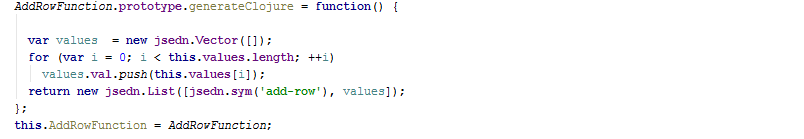
\includegraphics[width=36em]{./Figures/generate-clojure}
\begin{figure}[htbp]
\caption{Sample code generation of DSL from Grafterizer}
\label{fig:sample-jsedn}
\end{figure}
\end{center}
A sample generation of DSL from Grafterizer is shown in Figure \ref{fig:sample-jsedn}. We create a list that contains a symbol that represents a command followed by the input parameters to corresponding command. In this example the values that will be used to create a new row are passed as input parameters in a vector. Those values are derived from user interface using AngularJS. 




 
% % Chapter 5

\chapter{Evaluation} % Main chapter title
\label{Chapter5} % For referencing the chapter elsewhere, use \ref{Chapter5} 

\lhead{Chapter 5. \emph{Evaluation}} % This is for the header on each page - perhaps a shortened title
%----------------------------------------------------------------------------------------
In this section we discuss the evaluation of design and implementation of the work done in this thesis. We conduct feature evaluations and performance experiments on the prototype implementation of discussed solution components in specific experiment setups in order to derive conclusions.
\section{Feature Evaluation Aspects}
\subsection{Functional coverage}
The proposed solution should be able to deal with the standard open data preparation processes including data cleaning and RDF creation. We did a comparative analysis with the features supported by Grafter which was previously used to perform open data preparation, to ensure functional coherence and coverage of newly implemented system.  The prototype as of now supports following features in distributed computing manner and exposed to users using a DSL abstraction which is supported by dynamic transformation execution engine (Scalable-graftwerk). 
\begin{center}
	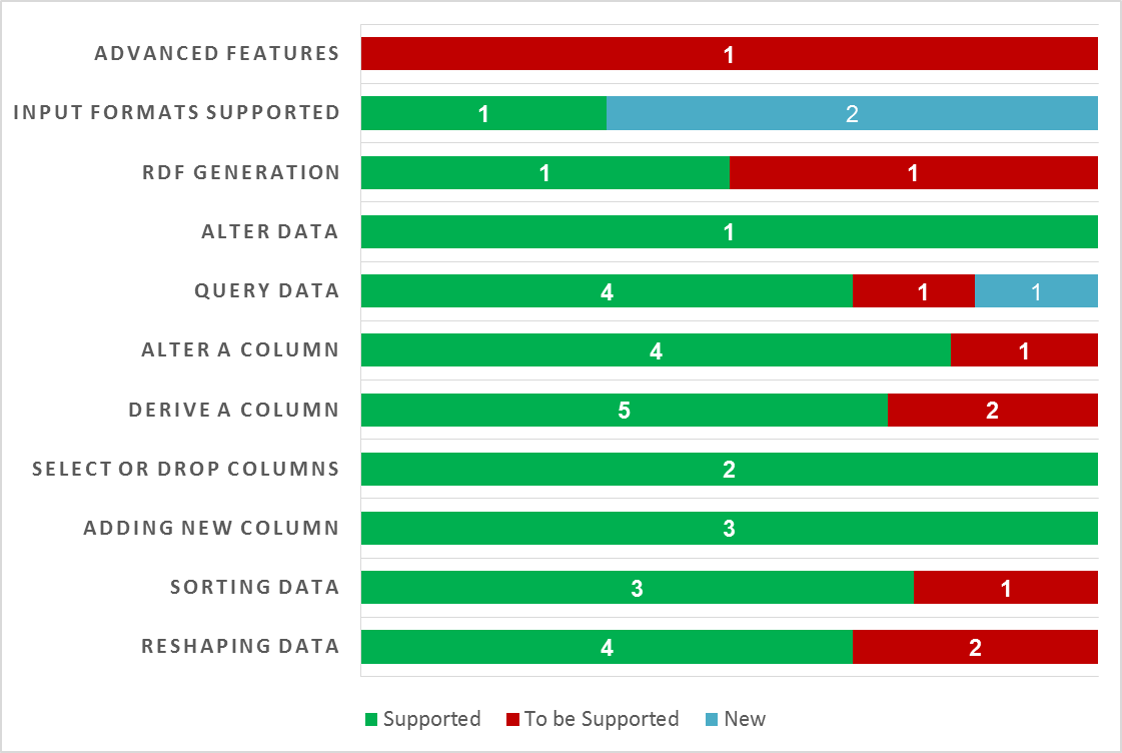
\includegraphics[width=38em]{./Figures/functional-coverage-new}
	\begin{figure}[htbp]
    \caption{Functional coverage of Scalable-graftwerk}
    \label{fig:func-coverage}
	\end{figure}
\end{center}
 In summary, implemented solution provides 39/47 major operations, i.e, ( ~83\% ), of requirements. Figure \ref{fig:func-coverage} shows that, most of the data cleaning functions are covered by implemented prototype as well as it can create RDF formats using simple mapping. In addition, Sparker provides more features such as querying using common logical expressions and supports more input formats.   Currently, it mainly lacks support of user-defined implementations of cleaning operations and pipeline functions due to the newly introduced context of distributed cleaning operations. However, provided that the main purpose of this solution is to support a user friendly, interactive data preparation, that can help to engage marginal audience in open data preparations, the currently implemented features satisfy user's requirements. 
% % how many implemented n wht is missing
% \subsection{Accuracy and consistency}
% how sampling helps? how consistent are sample n full execution vs other systems execution

\subsection{User friendliness}
User friendliness and a general purpose data preparation solution are important requirements of this solution. It is important to measure the user friendliness that is provided by the tool as it is expected to be used by users with various technical background. Grafterizer provides a very simple, easily understandable and intuitive interface with well explained documentation for  data cleaning and visualization, whereas other solutions such as Wrangler\cite{2011-wrangler}\cite{openrefine} require user to use domain-specific scripting to perform relevant data cleaning. This implicitly requires at least moderate level of technical knowledge which can be comparably tedious, time consuming and error prone. The user can use user interfaces in Grafterizer to perform data cleaning without manually entering cleaning scripts. 
\begin{center}
	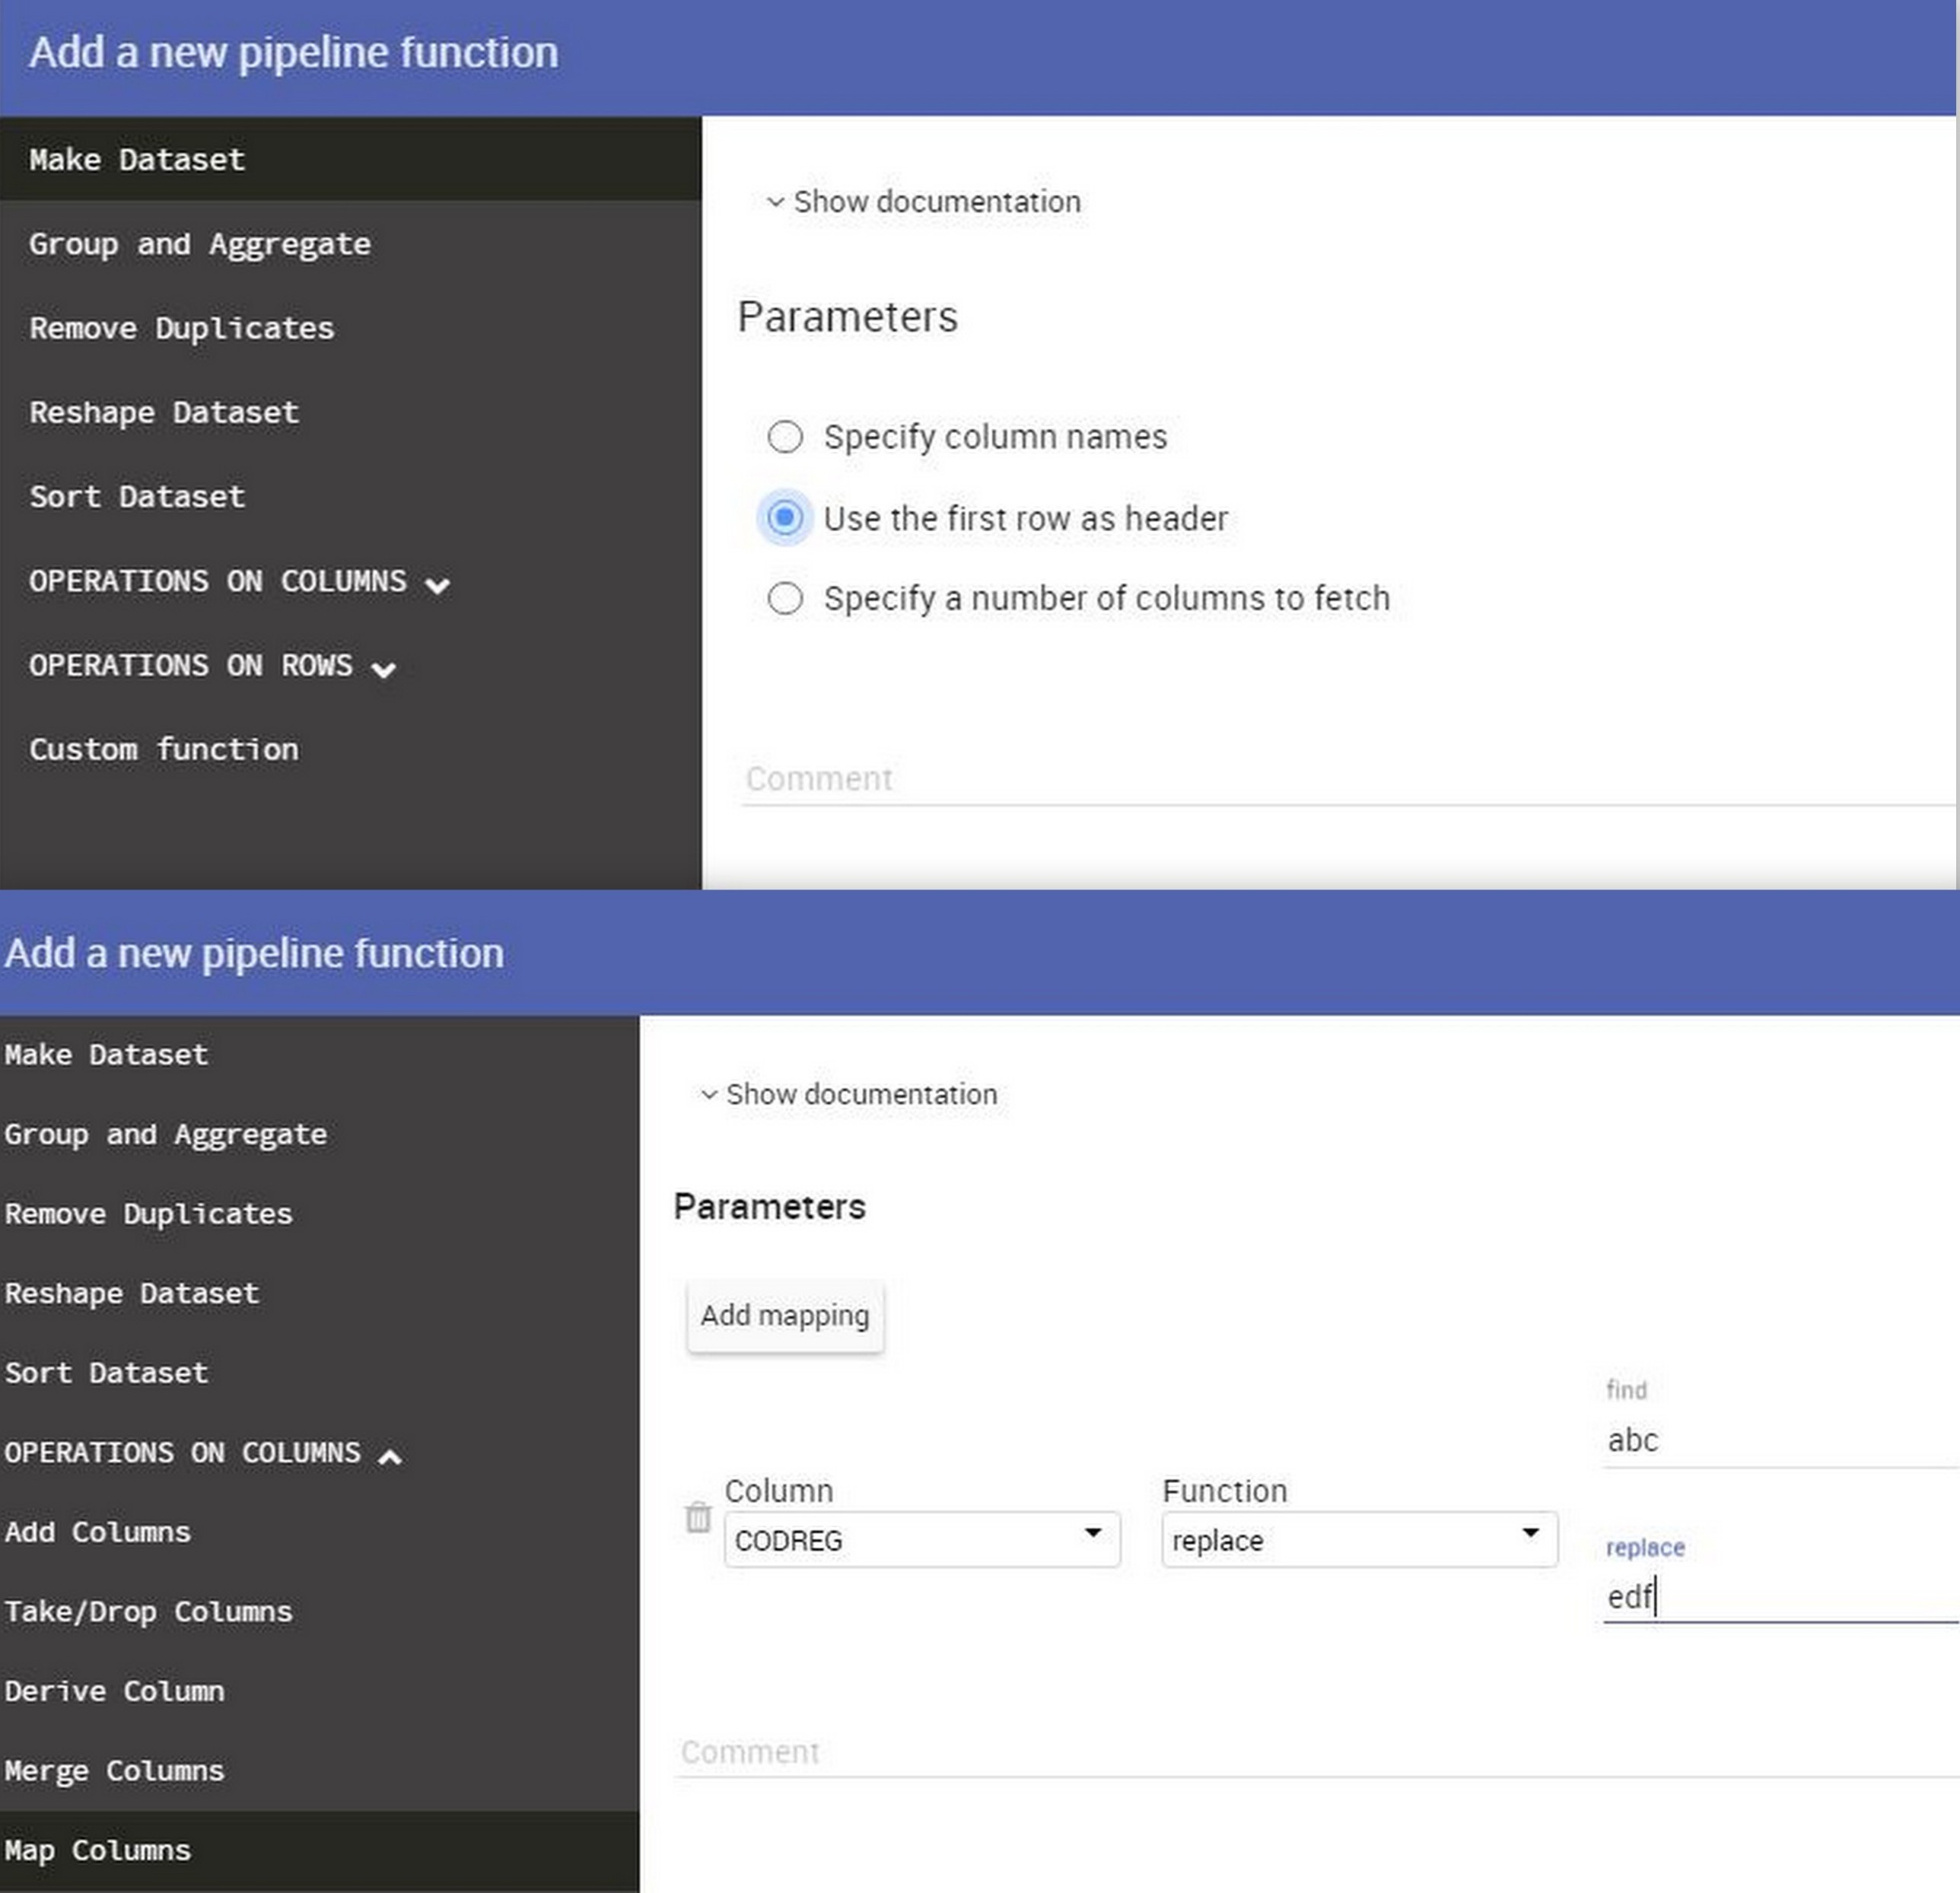
\includegraphics[width=38em]{./Figures/userinteraction}
	\begin{figure}[htbp]
    \caption{Grafterizer's interactive interface to create data cleaning pipelines}
    \label{fig:datacleaning}
	\end{figure}
\end{center}
The in-built script generator of Grafterizer converts user's input to a corresponding transformation pipeline command implicitly.  
\begin{center}
	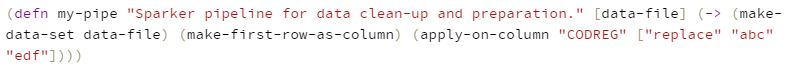
\includegraphics[width=38em]{./Figures/code-generated}
	\begin{figure}[htbp]
    \caption{Equivalent transformation pipeline script generated in Clojure}
    \label{fig:codegenerated}
	\end{figure}
\end{center}
This avoids unnecessary learning time and human errors in data preparation. Hence, Grafterizer is better suited than the other tools in terms of a complete interactive user interface that enables quicker data preparation.
\subsection{Interactivity and near-real-time response}
Provided that the treated data is large, a sample of data is created with the inputs of user to do interactive transformation. Since we consider incremental iterative transformations of large volume of data, with near-real-time response to have effective user interaction, sampling is essential.  Also, due to iterative transformation, the data being processed changes rapidly. This requires effective disposal of objects and garbage collection. For instance, Wrangler comparably performs slower due to lack of efficient object handling and leads to a longer response time when the tool is used continuously for longer period. It was noticeable, when larger data is loaded in Wranger\cite{2011-wrangler}, that the system took more than 15 seconds just to add a transformation pipeline in user interface, which later resulted in hindering user interaction holding user to wait for performing next data cleaning activity. Comparably, Grafterizer is very effective in terms of interactivity and near-real-time responsiveness since interactive transformation is efficiently performed on sample data and utilizing perfect garbage collection of under-lying system.
\section{Performance Evaluation Aspects}
In this section we evaluate the performance of implemented prototype in different experiments analyzing some critical aspects of proposed system, to draw conclusions of solution's viability from the results.
\subsection{Single Node Analysis}
\label{singlenode}
One of the important aspects Sparker gives is performing parallel execution of data preparation. Despite the system is hosted in a single machine, by exploiting in-memory computing and parallelization, Sparker can process large data faster than traditional processing applications. To analyze the performance of Scalable-graftwerk (using Sparker) in a single node, we created following sets of experiments that compares the performance of traditional processing application Graftwerk (using Grafter) and free-desktop version of Trifacta's Wrangler\footnote{https://www.trifacta.com/trifacta-wrangler/}. 

\textbf{Experimental setup}

Tests were conducted by sending HTTP requests to Scalable-Graftwerk and Graftwerk with corresponding data and transformation pipeline scripts then measuring the execution time taken to process the requests, whereas time elapsed to generate results from a pre-built transformation was recorded using stop watch in Wrangler which was installed as a standalone desktop application. Measuring execution time of pre-built transformation allows us to analyze the actual execution time, without considering the time taken to create transformation pipeline using UIs of these systems to come to a precise conclusion. All three systems were tested on same host computer with the following specifications:
\begin{itemize}
\item CPU - Intel Core i5-3210M CPU - 2.5 GHz - 4 cores
\item RAM - 8GM 
\item Operating System - Microsoft Windows 10 Home (64- bit Operating System, x64-based processor)
\end{itemize}
Scalable-Graftwerk was deployed using local-mode with \textit{ spark.master = local[*]} configuration. This allows Spark to utilize maximum parallelization of host computer.  

\textbf{Experiments and Results}

Experiments were performed on data of casualties from road accidents during 2005-2014 in Great Britain from Road Safety Data published on open data portal of Great Britain\footnote{https://data.gov.uk/dataset/road-accidents-safety-data}. The data is originally 94.9 MB, which is sampled into number of samples of smaller size and merged to create bigger data for the evaluation in the range of 9.3 MB to 120.7 MB. In total, we performed 12 experiments with different sized data-sets. A sample data transformation was created to perform data profiling, to remove two unnecessary columns and to do some word transpositions on specific columns. Equivalent transformation scripts were created for Scalable-Graftwerk, Grafwerk and Wrangler using corresponding interfaces. 
\begin{center}
	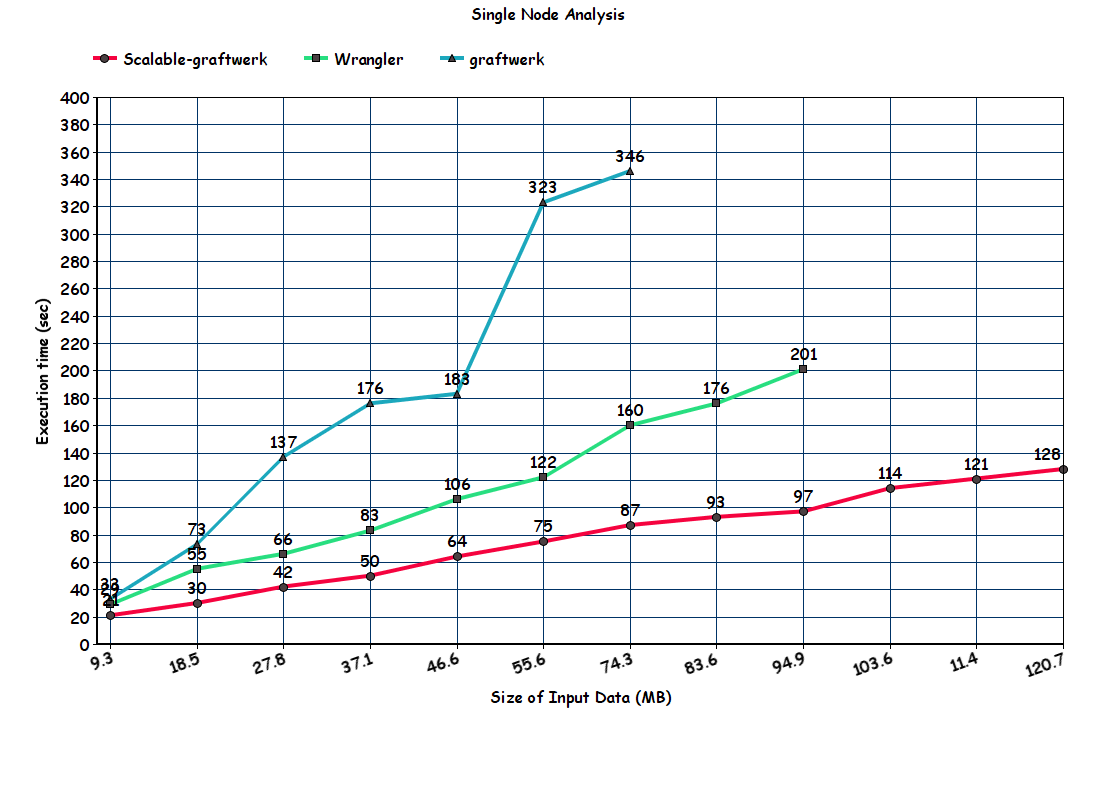
\includegraphics[width=38em]{./Figures/single-node}
	\begin{figure}[htbp]
    \caption{Single node analysis}
    \label{fig:singlenode}
	\end{figure}
\end{center}
Figure \ref{fig:singlenode} shows the execution time elapsed to process same data transformation on different sized data. Execution time of Wrangler and Scalable-graftwerk linearly increasing with the size of data.Wrangler has almost double the amount of execution time compared to Sparker,while Wrangler couldn't process data which is more than 100 MB in size. The maximum amount of data size that can be processed in Scalable-grafter converges to its allocated memory in local-mode. Whereas, Graftwerk with Grafter performed very slow compared to other two systems with roughly four times longer execution time than Sparker.

Another important fact to notice is Graftwerk, required a compulsory increase of heap size to process larger files. Figure \ref{fig:heapsize} shows the amount of heap size in GB, which was allocated during each experiments in all three systems. It is obvious to notice that, Grafter consumes large amount of heap memory to perform cleaning operations as a pipeline. When the process hits the allocated heap memory, the process stays idle or throws GarbageCollector(GC) GC overhead limit exceeded Exception. The reason can be since Grafter uses Clojure, which uses immutable objects, lack of effective garbage collection could have resulted in huge growth of heap memory to hold created data objects. It is noticeable that Graftwerk requires almost additional 1GB to process every 10 MB of input data, which is not feasible to process very large volumes of data. We could not continue the experiment for an input data which is more than 75 MB on Graftwerk. On the other hand, Scalable-graftwerk was allocated 1GB of memory and Wrangler used 1GB of memory throughout the experiments
\begin{center}
	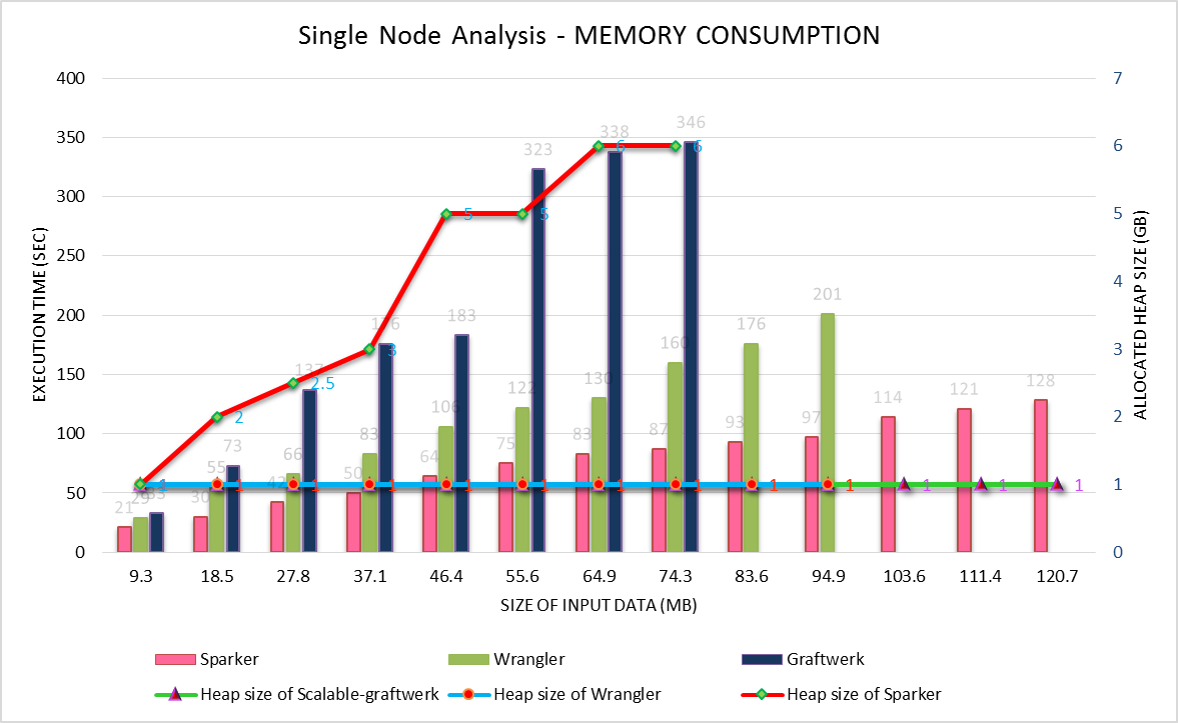
\includegraphics[width=38em]{./Figures/heapsize2}
	\begin{figure}[htbp]
    \caption{Heap sized used for Single Node Analysis}
    \label{fig:heapsize}
	\end{figure}
\end{center}
With the above experiments, it is safe to conclude that Scalable-graftwerk performs better in terms of capacity to process large files and faster execution time. 
\subsection{Cluster Analysis}
\textbf{Experimental setup}

The main goal of this thesis is to provide a scalable data preparation as a service. Thus, it is vital to investigate the scalability of proposed system. In order to measure the scalability of the system, we conducted few sets of experiments on Scalable-grafter. Scalable-grafter was deployed on a cluster using \textit{spark-submit}\footnote{http://spark.apache.org/docs/latest/submitting-applications.html} The cluster is managed by YARN resource manager\footnote{http://hadoop.apache.org/docs/current/hadoop-yarn/hadoop-yarn-site/YARN.html} in \textit{yarn-client mode} which suits interactive style of commands\footnote{http://blog.cloudera.com/blog/2014/05/apache-spark-resource-management-and-yarn-app-models/}. The cluster consists a master-slave architecture with following specifications:
\begin{itemize}
\item Master  Node : 	Intel Core i7 5820K 3.3GHz, 4 CPU Cores, 15 GB of RAM, 512GB of SATA SSD, Ubuntu 14.04 LTS
\item Worker Nodes : 4 x (Intel Core i7 5820K 3.3GHz, 12 CPU Cores, 64 GB of RAM, 480GB NVME SSD, 6*3 TB HDD, CentOS 7)
\end{itemize}
\begin{center}
	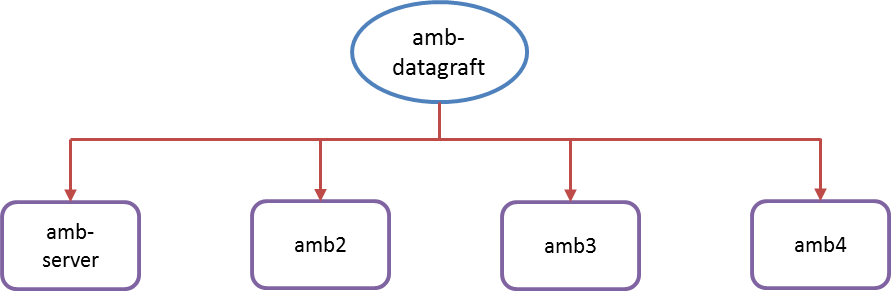
\includegraphics[width=38em]{./Figures/cluster}
	\begin{figure}[htbp]
    \caption{Structure of cluster}
    \label{fig:cluster}
	\end{figure}
\end{center}
Figure \ref{fig:cluster} depicts how the our test bed was setup.   two main parameters that can influence spark's performance are memory and CPU. Network I/O and Disk also affect Spark application's performance. However, YARN or Spark don't actively manage them till now. They are considered irrelevant in our experiments since we do not consider network provisioning time when creating SparkContext and reconcile data for these experiments. The performance of a Spark application like Scalable-graftwerk can be analyzed by tuning allocated memory and CPU. Focusing on scalability of the application, we decided to change the CPUs allocated to application and track performance accordingly.

\textbf{YARN Execution Model on a Cluster}

A Spark application consists of a single-driver process and a set of executor processes scattered across nodes on the cluster. The driver process  is responsible for the high-level control flow of work that needs to be done. The executor processes are responsible for executing this work, in the form of tasks. When a Spark application is submitted using park-submit using \textit{yarn-client} mode, a central master application request YARN resource manager for resource containers. YARN Manager informs master application with available resources according to request. The client's master application directly communicates containers to schedule jobs. 
\begin{center}
	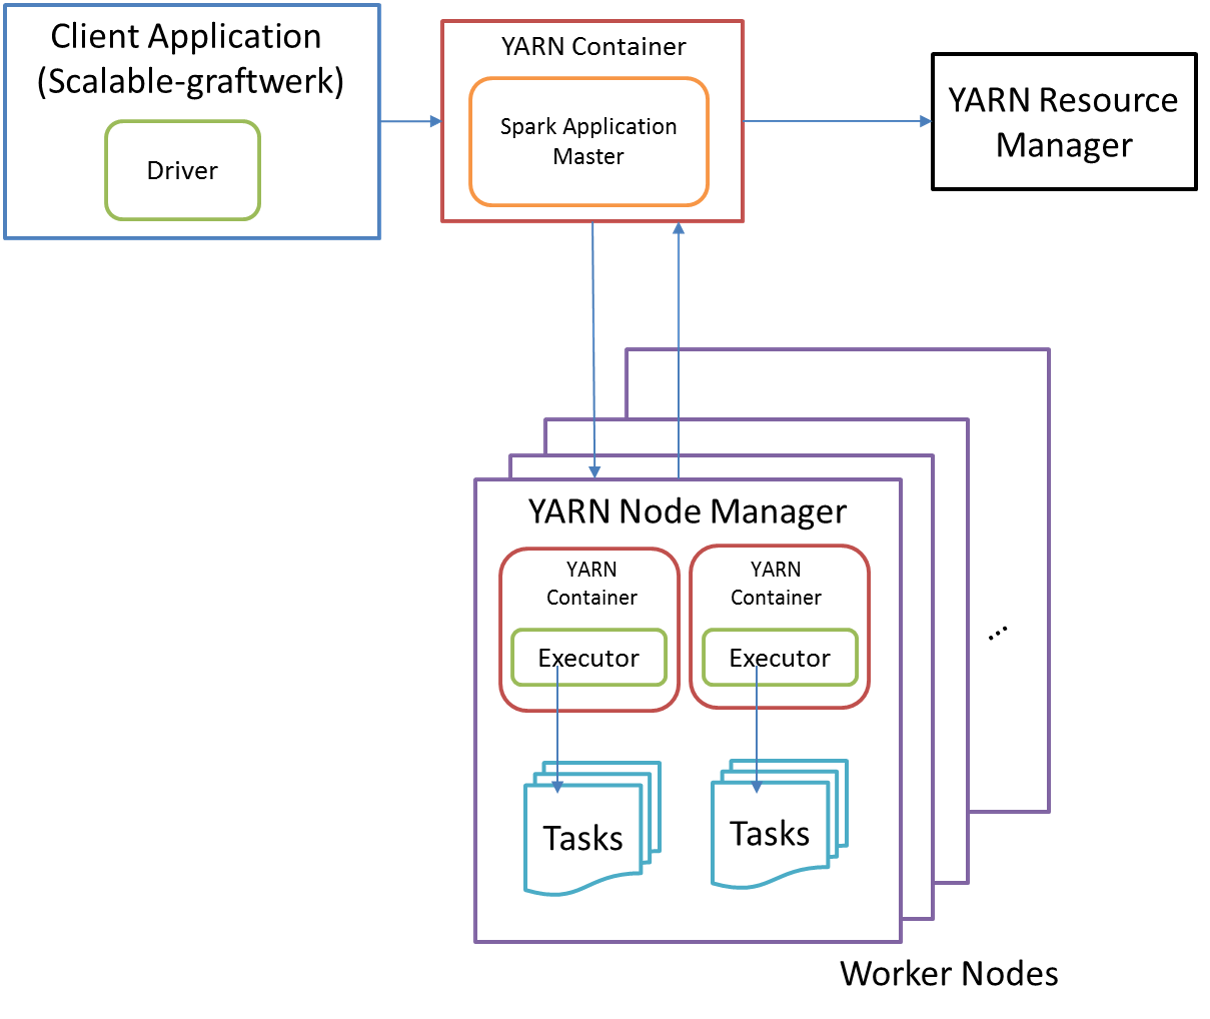
\includegraphics[width=33em]{./Figures/scalable-graftwer-in-yarn-cluster}
	\begin{figure}[htbp]
    \caption{Scalable-graftwerk's execution model on a YARN Cluster}
    \label{fig:yarn-cluster-model}
	\end{figure}
\end{center}
A Spark application can be manually tuned with respect to CPU by changing following properties
\begin{itemize}
\item Number of executors : 	An executor is a single JVM instance on a node that serves a spark application. An executor can run multiple tasks concurrently. Every executor has equal number of tasks and fixed amount of heap size
\item Number of cores used in a driver: Number of concurrent tasks an executor can run
\item Number of cores used in an executor:  Number of concurrent tasks an driver can run
\end{itemize}
These can be easily tuned by modifying spark configuration of the deployment to analyze the performance. 

\textbf{Experiments and Results}

All the experiments mentioned below are performed on Price Paid Data which contains information on all residential property sales in England and Wales that are sold for full market value and are lodged with Land Registry for registration\footnote{https://www.gov.uk/government/statistical-data-sets/price-paid-data-downloads}. The data-set contains information from 1st of January 1995 to the end of April 2016, that is 3.5 GB in size. We created a sample transformation that can load the file and make a data-set by using the first row values as column headers. The experiment was performed by sending HTTP Requests with generated data cleaning scripts and location of input file in HDFS. Figure \ref{fig:sample-pipeline} shows the cleaning script generated by integrated Grafterizer. 
\begin{center}
	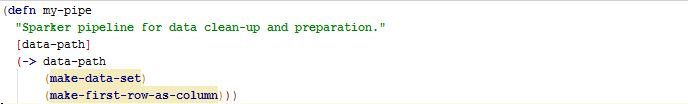
\includegraphics[width=35em]{./Figures/cluster-pipeline}
	\begin{figure}[htbp]
    \caption{Sample data cleaning script}
    \label{fig:sample-pipeline}
	\end{figure}
\end{center}
 Figure \ref{fig:spark-test-job} shows how the script generated in Figure \ref{fig:sample-pipeline} is executed in Spark. This involves 4 small tasks including fetching the first line, create a map of each line with an index and create new schema with provided logic and save the result as a CSV file in HDFS. It can be clearly seen the level of abstraction Scalable-graftwerk provides to execute Spark jobs eases the efforts of data workers.
\begin{center}
	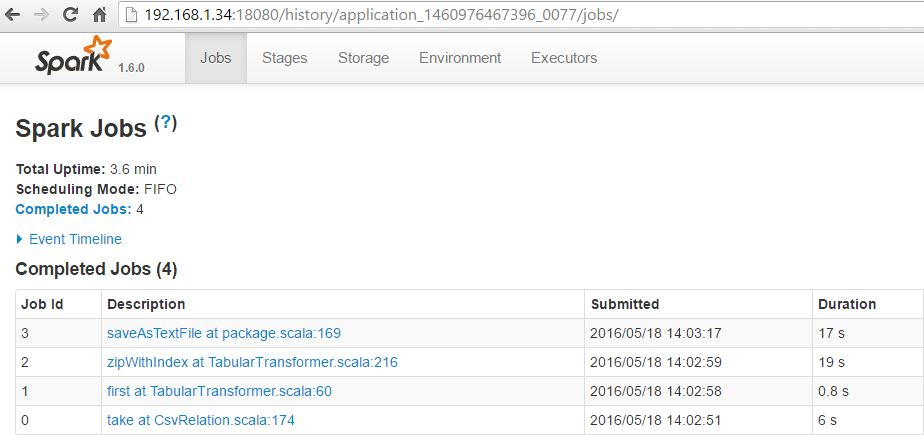
\includegraphics[width=38em]{./Figures/spark-job}
	\begin{figure}[htbp]
    \caption{Spark job of tested data cleaning pipeline}
    \label{fig:spark-test-job}
	\end{figure}
\end{center}
All the experiments below were executed with 
\begin{itemize}
\item Driver-memory : 4GB
\item Executor memory : 10GB
\item Default parallelism 
\end{itemize}
\subsubsection{\textbf{Scalability of Scalable-graftwerk}}
\label{scalability-exp}
The first experiment was conducted by deploying the application with a different number of executors with fixed number of driver cores and fixed number of executor cores. In this experiment we chose to use 2 driver cores and 2 executor cores per executor. We changed the number of executors from 1 to 20 to analyze the impact of number of executors in our application's performance. 
\begin{center}
	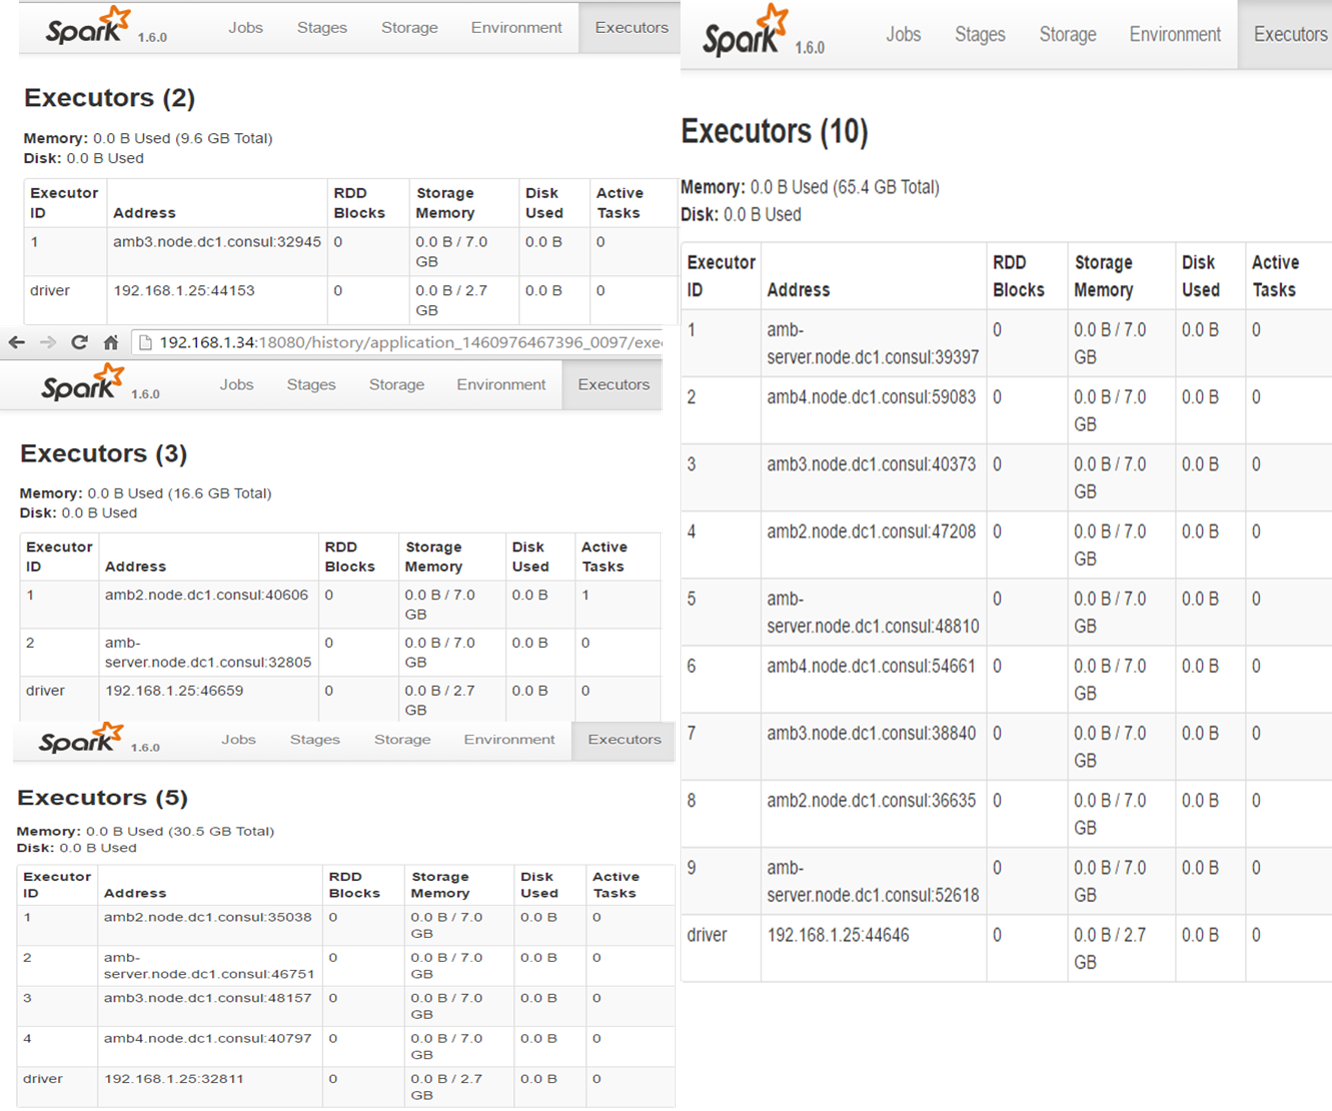
\includegraphics[width=35em]{./Figures/scale}
	\begin{figure}[htbp]
    \caption{Scalability of Scalable-graftwerk on distributed nodes}
    \label{fig:scale}
	\end{figure}
\end{center}
Figure \ref{fig:scale} shows that Scalable-graftwerk can automatically scale-out on different nodes when number of executors are changed. This lets the application to utilize the resources available on a cluster
\begin{center}
	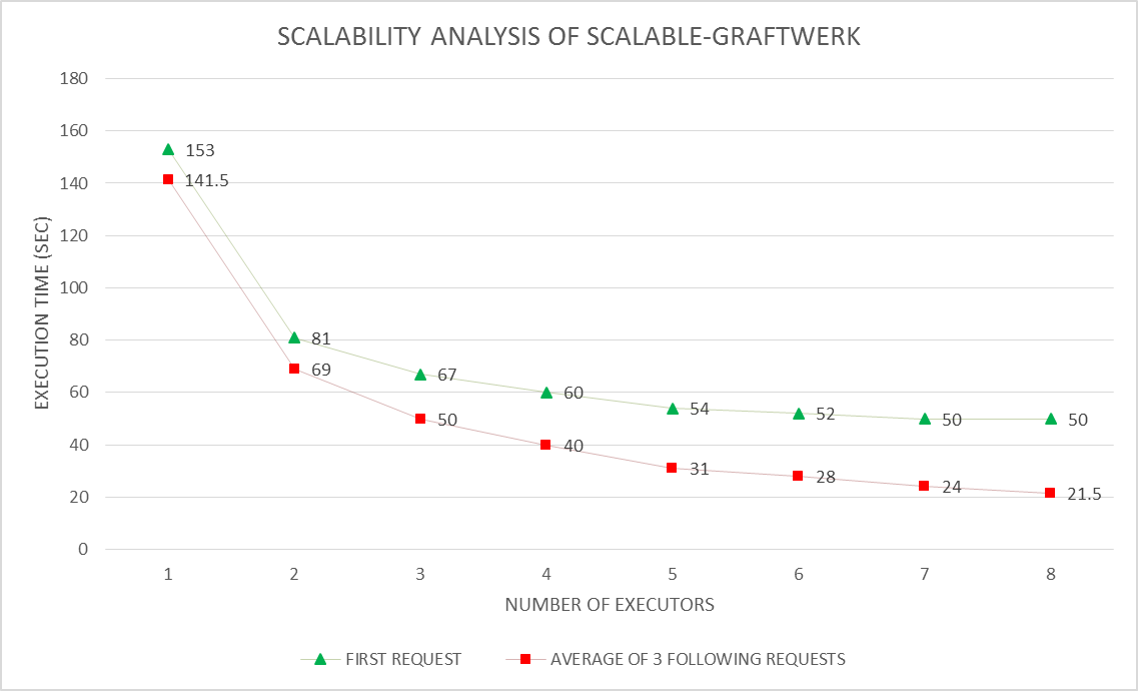
\includegraphics[width=38em]{./Figures/executors2}
	\begin{figure}[htbp]
    \caption{Scalability analysis of Scalable-Graftwerk}
    \label{fig:executors}
	\end{figure}
\end{center}
We noticed that there is a significant difference between execution time of the first request after a SparkContext is initialized and requests follow the first request, while the difference between following request were significantly small (0 -2 seconds). Reasons for this difference can be initialization of tasks in background that are required for execution of a job. Since, we are providing Scalable-graftwerk as a service, the execution time of first request seldom impacts on application performance, since the service is expected to be available when a user starts a data preparation process. We focus more on the performance on interactive, and iterative operations. Thus, we recorded the execution time of first request and average of 3 following request for this set of experiments. Figure \ref{fig:executors} shows the execution time elapsed for different number of executors. The main observations we noticed from these experiments are, 
\begin{itemize}
\item Execution time of a job is improved with maximum difference of 125 seconds (141.5 to 15.5) with 1 to 20 executors. 
\item Performance of application increases exponentially for both first request and average of following request till a minimum execution time of executed job is reached ( met with 8 executors ).  
\item Execution time of first request starts to increase from 9 executors (after minimum required execution time is met) and remains almost unchanged after 15 executors.
\item Execution time of average of following requests is nearly unchanged with decrease of maximum of 5 seconds from 9 executors to 20 executors
\end{itemize}
It can be clearly seen that performance of the application increases till a minimum threshold execution time is reached. When more executors are provided, it creates multiple virtual cores that can equally execute a job in parallel. The more executors are allocated, the less work-load is shared per executor. However, parallelism of tasks plays a significant role in Spark application's execution time, which we don't focus in this experiment. We notice that a job lasts at least for a minimum amount of time, regardless of increase of executors with unchanged parallelism. We refer this as the minimum execution time of a Spark job for a given parallelism. Once the minimum threshold of execution time of a job is reached execution time of a first request increases. When more executors are used it requires initialization and coordination of background tasks in more executors, while the process requires at least a minimum amount of execution time. This reasons the behavior of execution time of first request. Through this experiment we conclude that Scalable-graftwerk is scalable with default parallelism until the minimum execution time of corresponding Spark job is reached. 
 
\subsubsection{\textbf{Concurrent execution of multiple tasks}}
Apart from scalability experiment discussed in Section \ref{scalability-exp} , we conducted another experiments to analyze whether we can  improve the performance of Scalable-graftwerk further. We set up more sets of experiments by changing the number of cores allocated for each executors from 1 to 12, with fixed number of executors and fixed number of driver cores. 

To analyze the behavior of concurrent task execution, we conducted 3 sets of experiments with 2, 5  and 7 executor instances and 2 cores for driver process. Since the average execution time of requests after the first request represents application's performance than execution time of first request after a SparkContext is initialized, we recorded the average execution time of 3 requests after the first request of an initiated context.
\begin{center}
	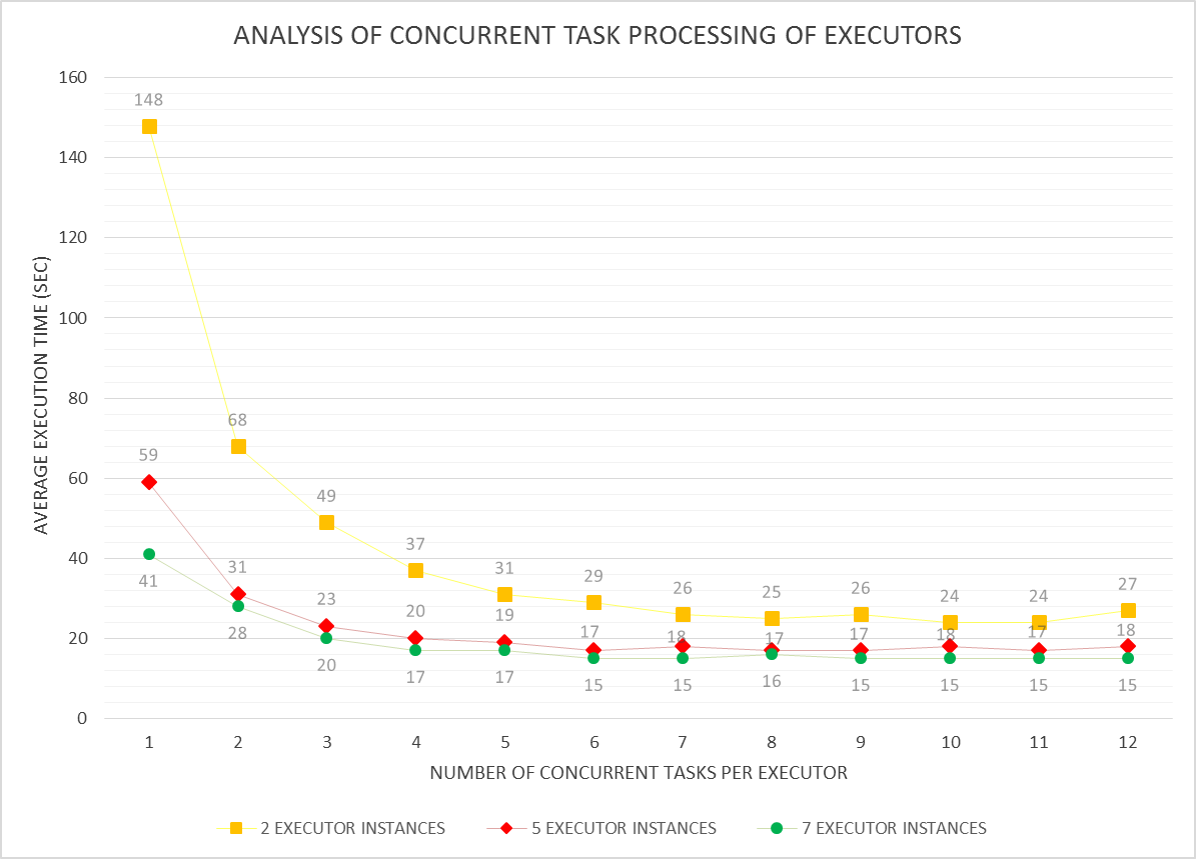
\includegraphics[width=38em]{./Figures/executor-cores2}
	\begin{figure}[htbp]
    \caption{Analysis of concurrent task processing of executors}
    \label{fig:executor-cores}
	\end{figure}
\end{center}
Figure \ref{fig:executor-cores} illustrates the observations of these experiments.  It is clear that, there is an exponential growth of performance from 1 core to 6 cores per executor. From 6 executors to 12 executors the performance is not significantly improved. It is rather unchanged with small differences ( 2 seconds ). The reason behind this behavior is HDFS has some performance limitations of concurrent task processing. When more than 5-6 concurrent tasks are executed on an executor process, the performance of the application is not improved as expected, since an overhead of processing too many concurrent tasks are introduced on HDFS. It is wise to keep the number of concurrent tasks (executor-cores per executor) below this limit for the optimal performance of this application.  

Moreover, the improvement in execution time increases with indirect-proportion of number of executors. Further it can be clearly seen, the impact of having more executors improve performance of the application, regardless of parallelization of concurrent tasks per executor. This behavior assures the claim made from previous experiment in Section \ref{scalability-exp}. 

As mentioned earlier, the other parameter that can be tuned on a Spark application is number of driver-cores. We didn't conduct any experiments to study behavior of driver-cores, since we focus on scalability and parallization of distributed executors, whereas driver process always run on a single machine. 

Overall, through all experiments mentioned in this section, Scalable-graftwerk can scale-out with more executors according to the cluster and number of executors requested. It can improve the performance until the minimal execution time for given parallelism is reached. Further, Scalable-graftwerk's performance can further be improved by having 5-6 executor cores per executor.  


 
%% Chapter 6

\chapter{Conclusion} % Main chapter title
\label{Chapter6} % For referencing the chapter elsewhere, use \ref{Chapter6} 

\lhead{Chapter 6. \emph{Conclusion}} % This is for the header on each page - perhaps a shortened title

%--------------------------------------------------------------------------------------------------------------

By using suitable techniques and best practices with appropriate data ingestion and programming model, we have provided an innovative Scalable Open Data Transformation as a Service, that can be easily used by open data workers including users without high technical skills. We designed a system architecture and process work-flow that enables an automated, integrated solution to provide interactive open data transformation. We summarize our main features and contributions as below:
\begin{itemize}
\item Batch processing using in-memory processing for iterative and interactive processing of large files - Through our literature study and a descriptive analysis, we showed that batch processing suits to process the large stored files to perform data cleaning operations to produce precise results. Further, in-memory processing suits iterative and interactive processing well by eliminating high I/O for storing and loading intermediate results.
\item Distributed open data preparation functions using Spark - We created a scalable open data preparation framework that has an interchangeable data abstraction that can process tabular data and convert to graph using Apache Spark's libraries and extensions. Moreover, we implemented complex data cleaning operations displayed in Table \ref{fig:features} and provided simple APIs that can be easily integrated and used to create pipelines of data transformation operations. This reduces the overhead of learning distributed processing of tabular and graph-based data. 
\item Dynamic execution engine of data transformation - We built an automated, transformation execution engine by using a dynamic language Clojure. It allows to create a data transformation as pipelines of transformation functions, built using a DSL that extends distributed data preparation techniques. This engine is exposed via Web Service APIs, that allows interoperability and loose coupling between client and data preparation system. This engine is 4x times faster than traditional data cleaning system in a single hosted machine, by utilizing parallelization. In addition it is capable of processing larger input data, where the maximum size of input file converges to allocated memory. 
\item Scalable open data preparation as a Service - We created solution that can be deployed on a distributed environment as a service. Through the evaluation, we show that it can scale-out or scale-in according to allocated  executor resources. Secondly, we present that the maximum performance of the solution can be achieved by scaling-out with more executors. However, every job takes a minimum amount of execution time according to current parallelism. The performance can be further improved by allocating more executor-cores to utilize concurrent execution of tasks. Despite, maximum threshold of allocated executor-cores is 5-6 that can improve performance, since executor-cores passing the maximum threshold introduce overheads of processing concurrent threads on HDFS. By utilizing distributed shared memory and cluster of computing resources our solution can process large volume of input data, such that the size of maximum input data that can be processed converges to the distributed shared memory that can be allocated.
\item Automated, integrated solution to provide interactive open data transformation - We demonstrated an integration of our scalable data transformation as a service, to provide near-real-time interactive data cleaning and RDF creation. By providing improved work-flow that allows sampling and caching that process is optimized and capable of guiding user to perform data preparation of large data. Finally, this is the only solution as a service that provides interactive platform to build transformation pipeline and data cleaning and RDF generation altogether as a single ended solution. 
\end{itemize}
Finally, as secondary contributions we, we provide open sourced implementations of our solution that is designed and developed using component based architecture. Hence, they can be used as a service or as separate solution component by user. Further, it is beneficial to users who would like to take advantages from scalable open data transformation without using service based solution to avoid security and policy issues, by simply deploying in local cluster environment. We have also implemented most sought after data cleaning requirements that are not provided by DataFrame API, that can be reused by relevant users. 

Future work of this research could include implementation of completely featured RDF mapping and generation. Flexibility and customization of data cleaning functions are important to meet technically oriented users. Our DSL should be improved further to allow customization of data cleaning functions. Since this solution involved multiple solution components, providing an installation pack or a container that consist all solution components installed is essential for users to make advantage of our solution instantly.  

% Through use of appropriate use of technology and techniques, we have provided an innovative and user friendly solution to scalable open data preparation. We designed a system architecture and a process that enable the a service based open data transformation that is automated interactively guide user to prepare linked data from raw data. We summarize its main contributions below:
% \begin{itemize}
% \item Data ingesting technique and Programming model to process iterative and interactive operations
% \item distributed open data preparation techniques and scalable open data preparations as a service x time faster than traditional processing and capacity to process converge to allocated memory size
% \item The settings for the maximum performance of the application. 
% \item Automated, integrated solution as a service for interactive open data transformation. 
% \item Work-flow optimization for interactive processing of large data. 
% \end{itemize}

% Futurework, 
% cont impl of adv rdf
% improve dsl to support custom function
% backend cluster improvements
% provide installation pack


% batch produces accurate result, near-real-time
% spark's prog model n rdd helps
% major impediment eliminated
% x times faster in local n cluster
% user friendly
% unique 
%\input{./Chapters/Chapter7} 

%----------------------------------------------------------------------------------------
%	THESIS CONTENT - APPENDICES
%----------------------------------------------------------------------------------------


\addtocontents{toc}{\vspace{2em}} % Add a gap in the Contents, for aesthetics

\backmatter

%----------------------------------------------------------------------------------------
%	BIBLIOGRAPHY
%----------------------------------------------------------------------------------------

\label{Bibliography}

\lhead{\emph{Bibliography}} % Change the page header to say "Bibliography"

\bibliographystyle{unsrtnat} % Use the "unsrtnat" BibTeX style for formatting the Bibliography

\bibliography{Bibliography} % The references (bibliography) information are stored in the file named "Bibliography.bib"

\end{document}